\chapter{Grundlagen}
\label{chapter:grundlagen}

In diesem Kapitel werden die für diese Arbeit relevanten theoretischen und konzeptuellen Grundlagen beschrieben. Begonnen wird mit einer kurzen Einführung in das Brettspiel Patchwork. Anschließend widmet sich dieses Kapitel der Spieltheorie, einem mathematischen Bereich, der bei der Modellierung und Analyse von Entscheidungssituation verwendet wird. Dann wird der Minimax-Algorithmus betrachtet, der den grundlegenden Algorithmus für einen in dieser Arbeit implementierten Computergegner darstellt. Anschließend werden die Grundlagen für zwei weitere Computergegner geschaffen, indem die Theorie von \acl{MCTS} und AlphaZero erläutert wird. Abschließend werden interaktive System erläutert, die für die Gestaltung der Benutzerschnittstellen und Spielererfahrung der Computerumsetzung des Brettspiels wichtig sind.

\section{Brettspiel Patchwork}
\label{chapter:brettspiel-patchwork}

\begin{wrapfigure}{r}{0.28\textwidth}
    \centering
    \vspace*{-1.3cm}
    \vspace*{-0.75cm}
    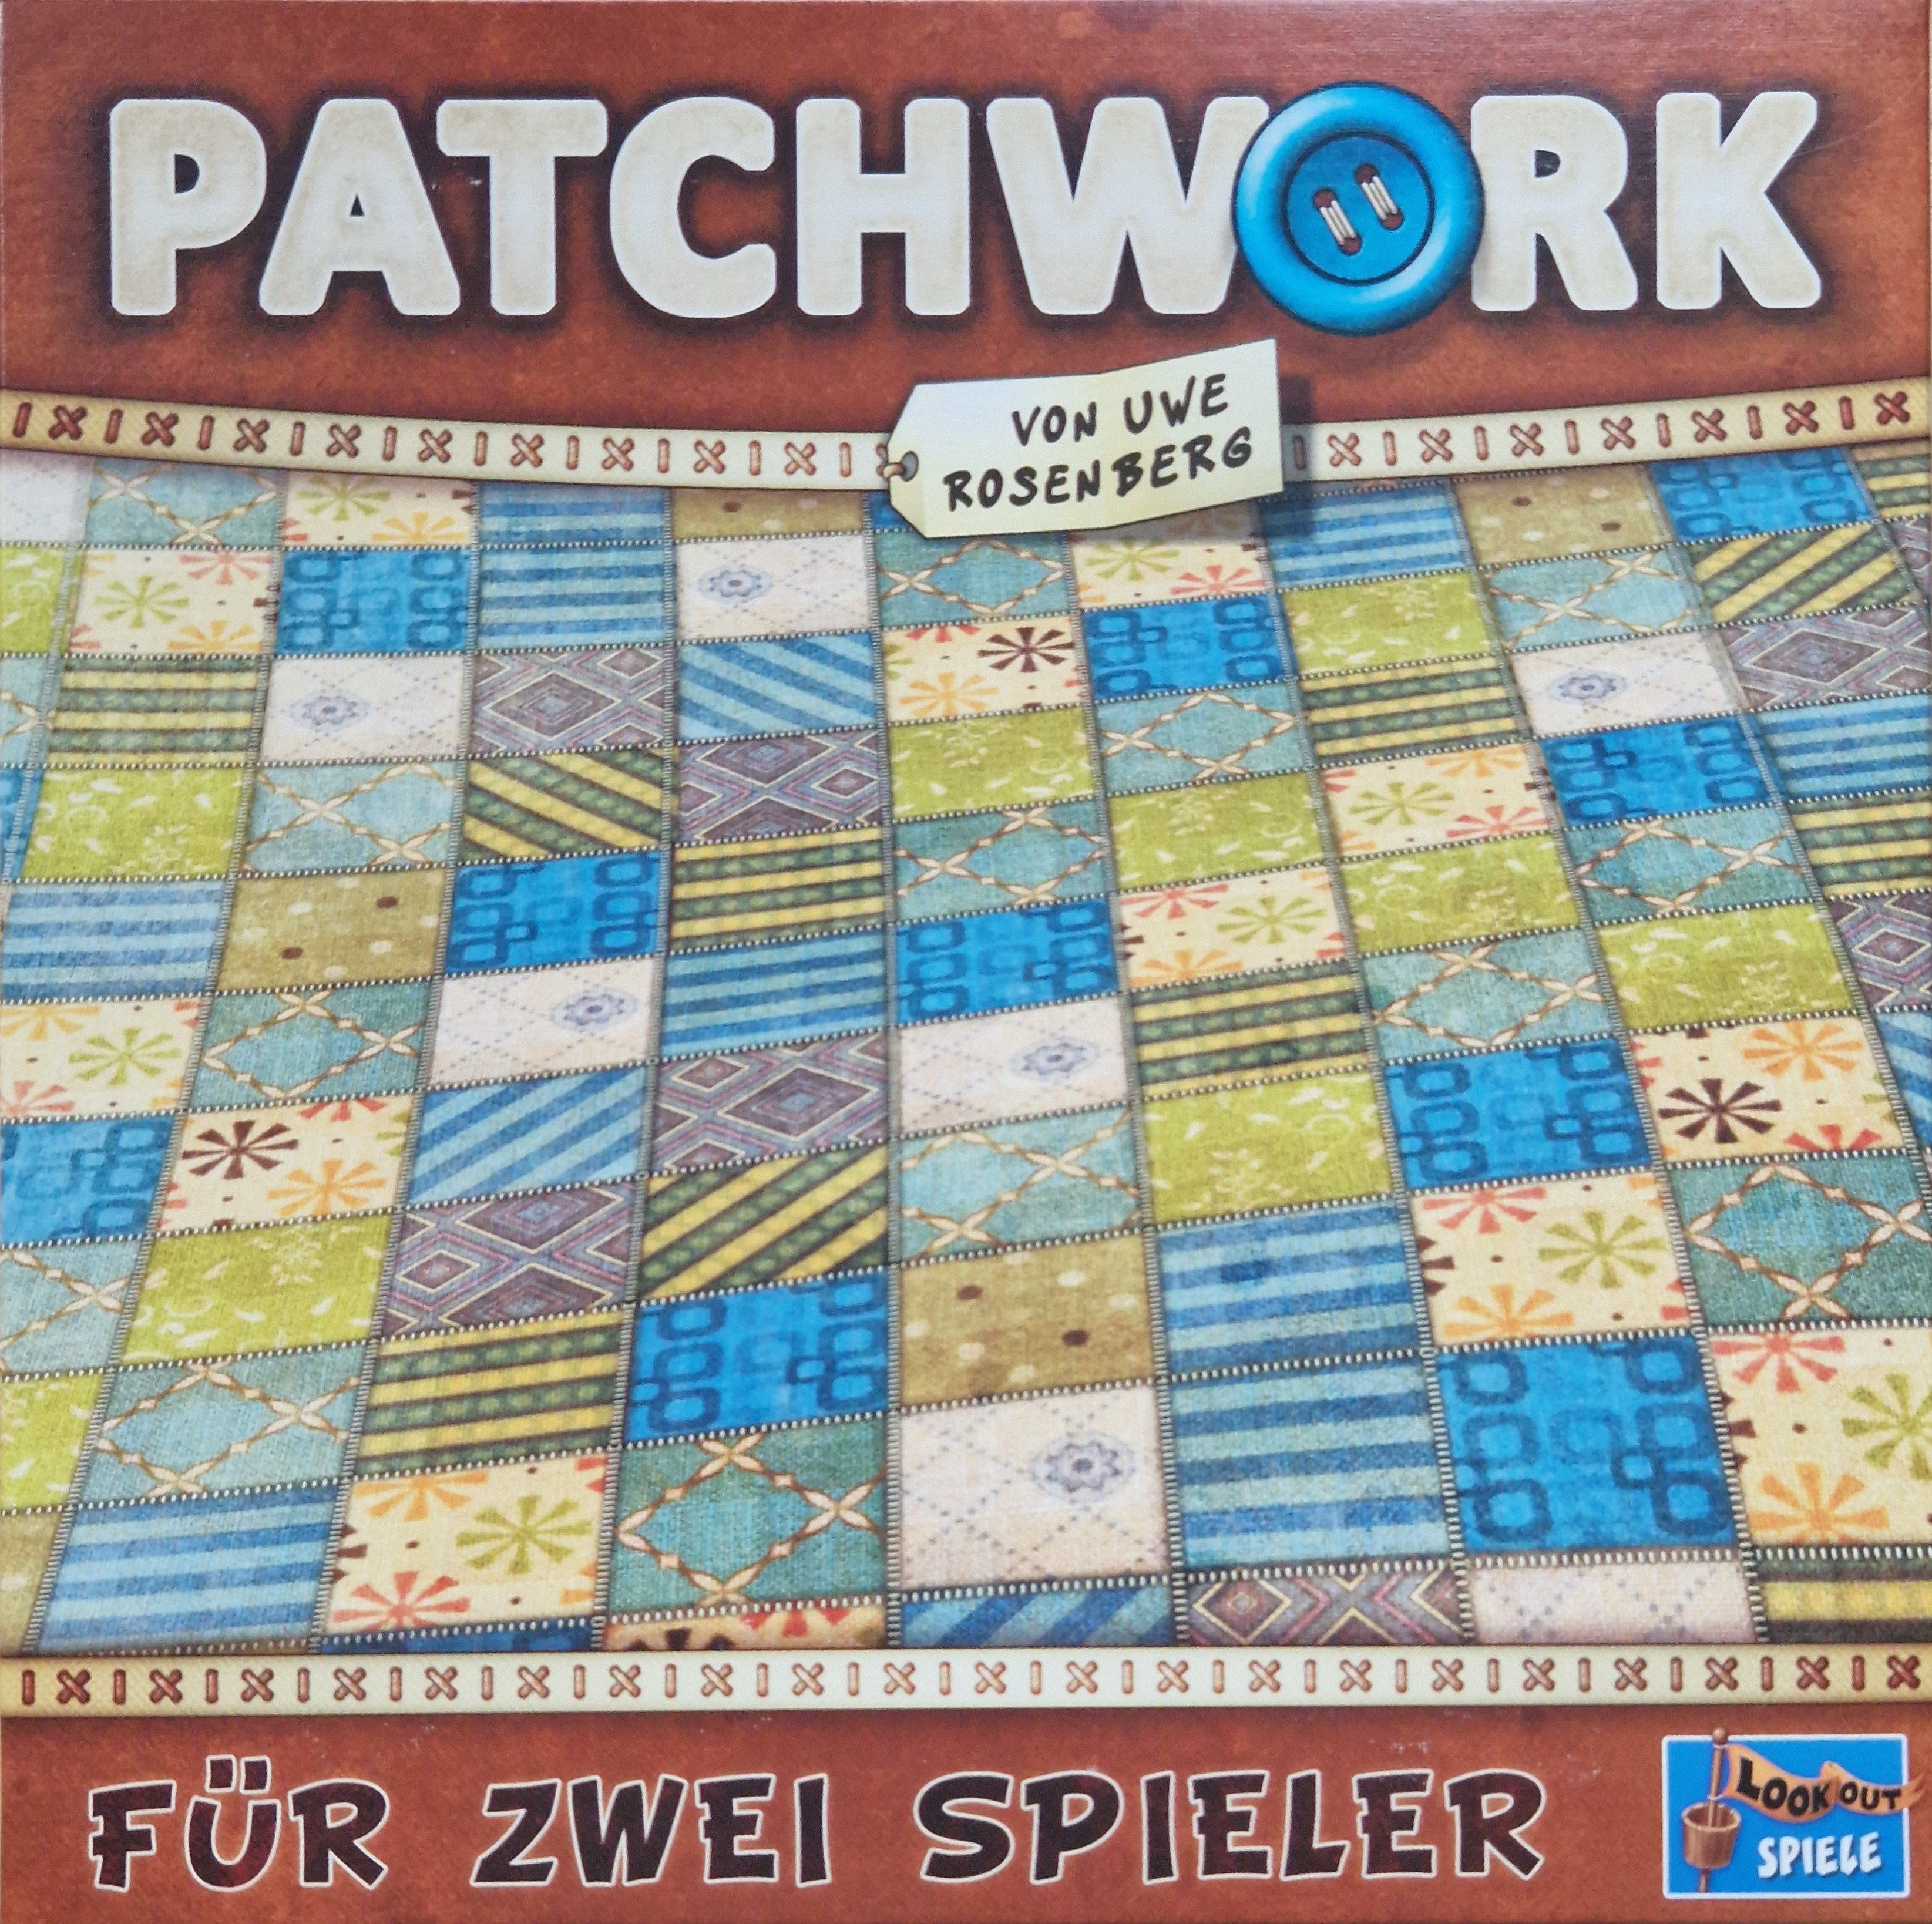
\includegraphics[width=0.265\textwidth]{res/pictures/assets/patchwork-cover.png}
    \caption[Cover von Patchwork]{\unskip}
    Cover von Patchwork
    \label{fig:patchwork-cover}
    \vspace*{-0.75cm}
\end{wrapfigure}

Patchwork ist ein Brettspiel von Uwe Rosenberg, das 2014 bei Lookout Spiele erschienen ist. Bei dem Brettspiel spielen zwei Spieler vom Alter 8 Jahre und aufwärts gegeneinander, wobei ein Spiel in der Regel ungefähr 30 Minuten lang ist \cite{LookoutSpielePatchwork}. Bei dem Brettspiel gestalten zwei Spieler jeweils eine eigene Decke aus Stoffresten, Flicken und Knöpfen, der Technik entsprechend, die der Titel vorgibt. \cite{SpielDesJahresPatchwork}

Das Ziel der Spieler ist mit den gegebenen Stoffplättchen unterschiedlicher Formen und Größen die vorgegebene Fläche zu füllen. Das Puzzlespiel erfordert taktisches Gespür, da die Flickenauswahl die Zugfolge und auch die Flickenauswahl des Gegenspielers beeinflusst. Immer können die Spieler jedoch nicht die gewünschten Flicken verwenden, da diese mit der Spielwährung Knöpfe aus der eigenen Kasse bezahlt werden müssen. An die begehrten Knöpfe kommen die Spieler über die bereits eingearbeiteten Flicken, welche Knöpfe auf sich abgebildet haben. Je mehr dieser Knöpfe auf der eigenen Decke abgebildet sind, desto höher das Einkommen an Knöpfen. Wer am Schluss des Spiels die meisten Knöpfe erwirtschaftet und seine Decke gut bestickt hat, gewinnt den Nähwettstreit. \cite{SpielDesJahresPatchwork}

\vspace*{-10cm}
\pagebreak

\section{Spieltheorie}
\label{chapter:spieltheorie}

Die Spieltheorie stellt einen theoretischen Ansatz dar, um Situationen zwischen Akteuren zu analysieren und deren strategisches Handeln zu verstehen. Das Ziel ist das Ermöglichen der optimalen Entscheidungsfindung für Akteure in strategischen Kontexten, indem verschiedene Modelle und Szenarien entworfen werden und deren wahrscheinliche Ausgänge prognostiziert werden. \cite{2024.GameTheory}

Jede Menge von Zuständen, bei denen das Ergebnis von den Handlungen von einer bestimmten Anzahl von Entscheidungsträgern abhängig ist, ist ein \emph{Spiel} \cite{2024.GameTheory}. Die an einem Spiel teilnehmenden Entscheidungsträger werden als \emph{Spieler} bezeichnet. Das Spiel unterliegt bestimmten \emph{Regeln}, die die Spieler einhalten müssen \cite[S. 1]{2014.GameTheoryThroughExamples}. Auf Basis dieser Regeln ist ein \emph{Zustand} nun eine Situation, in der Spieler \emph{Entscheidungen} treffen. Durch das Treffen einer Entscheidung, werden \emph{Aktionen} ausgeführt, welche einen neuen Zustand erzeugen \cite[S. 1]{2014.GameTheoryThroughExamples}. Jeder Zustand kann für einen Spieler mit einem \emph{Wert} beschrieben werden. Die Differenz dieser Werte zwischen dem vorherigem Zustand und dem neuem Zustand wird als \emph{Auszahlung} der Aktion bezeichnet \cite{2024.GameTheory}. Hat eine Aktion also eine positive Auszahlung für einen Spieler, so befindet sich dieser Spieler nach dem Treffen der Entscheidung in einer besseren Situation als zuvor. Zusätzlich zu den normalen Zuständen, gibt es Situationen, in denen das Spiel endet, sogenannte \emph{Endzustand} \cite[S. 53]{2014.GameTheoryThroughExamples}. Weiterhin beginnt jedes Spiel in einem \emph{Startzustand} \cite[S. 53]{2014.GameTheoryThroughExamples}.

Spiele können nach mehreren Kriterien charakterisiert werden. Ein Spiel ist \emph{kooperativ}, wenn die Spieler gemeinsam versuchen auf das gleiche Ziel hinzuarbeiten und \emph{kompetitiv} andernfalls, \dash die Spieler verfolgen nicht das gleiche Ziel \cite{2018.CooperativeGames}. Ein \emph{sequenzielles} bzw. \emph{zugbasiertes} Spiel ist ein rundenbasiertes Spiel, wo die Spieler nacheinander ziehen \cite[S. 251]{2018.SequentialGame}. \emph{Strategiespiele} erfordern die langfristige Planung des Vorgehens, um in dem Spiel erfolgreich zu sein. Diese Spiele zeichnen sich meist auch dadurch aus, dass keine oder kaum Zufallselemente im Spiel vorkommen. Generell sind Zufallsprozesse in Spielen aber erlaubt. Außerdem existieren Spiele mit \emph{perfekter Information}, bei denen alle Spieler zu jedem Zeitpunkt während des Spiels Zugriff auf alle Informationen haben, die zu dem derzeitigen Zustand geführt haben und diesen Zustand vollständig charakterisieren \cite[S. 156]{1194.SearchAndAiInGames}. Des Weiteren gibt es den Begriff der \emph{vollkommenen Information}, der aussagt, dass allen Spielern alle Spielregeln und auch möglichen Spielzüge bekannt sind \cite[S. 1]{2017.AlphaBeta}.

Bei Spielen mit perfekter Information ohne vollkommene Information ist zwar der Zustand des Spiels für alle Spieler bekannt, aber ein Spieler kann möglicherweise eine Aktion ausführen, von der die anderen Spieler vorher nicht wussten, dass sie möglich ist. Dahingegen sind alle Aktionen bei Spielen mit vollkommener Information aber ohne perfekte Information bekannt, aber der derzeitige Zustand nicht für alle Spieler komplett ersichtlich. \emph{Nullsummenspiele} sind solche Spiele, bei denen der Verlust des Wertes bei einem Spieler gleich dem Gewinn des Wertes bei einem anderem Spieler entspricht \cite{2022.ZeroSumGame}. Somit ergibt sich als Endergebnis für den Gesamtwert eine Nullsumme.

Auch die Konvergenz von Spielen wird in der Spieltheorie betrachtet. Eine Aktion von Zustand $A$ nach Zustand $B$ ist eine umwandelnde Aktion, wenn in einem Spiel, das von Zustand $B$ ausgeht keine Konfiguration von Spielteilen auftreten kann, welche in einem Spiel hätte auftreten können, welches zur Konfiguration von Spielteilen in Zustand $A$ geführt hätte \cite[S. 157]{1194.SearchAndAiInGames}. Nimmt man zum Beispiel ein Spiel, bei dem das Ziel ist, alle Felder auf einem Spielbrett auszufüllen, so ist jede Aktion, die ein weiteres Feld ausfüllt, eine konvergierende Aktion, falls es keine Aktionen gibt, die Felder wieder entleeren. Teilt man nun alle Zustände in die verschiedenen Zustandsklassen ein, beispielsweise die Anzahl von ausgefüllten Feldern auf dem Spielbrett, so lässt sich ein gerichteter Graph definieren, deren Knoten durch die umwandelnden Aktionen verbunden werden. Ein Spiel konvertiert genau dann gegen einen Endzustand, wenn für alle Kanten von der Klasse $A$ nach $B$ mehr Knoten in $A$ existieren als in $B$, \dash immer weniger mögliche Zustände im späteren Verlauf des Spiels existieren \cite[S. 157]{1194.SearchAndAiInGames}. Das Spiel divergiert, falls das Gegenteil der Fall ist, also im späteren Verlauf immer mehr mögliche Zustände existieren \cite[S. 157]{1194.SearchAndAiInGames}. Es ist auch möglich, dass keiner der beiden Fälle auftritt. Die Konvergenz und Divergenz von Spielen ist in den Abbildungen \ref{fig:spieltheorie-konvergenz} und \ref{fig:spieltheorie-divergenz} visualisiert.

\begin{figure}[!ht]
    \centering
    \begin{minipage}{.385\textwidth}
        \centering
        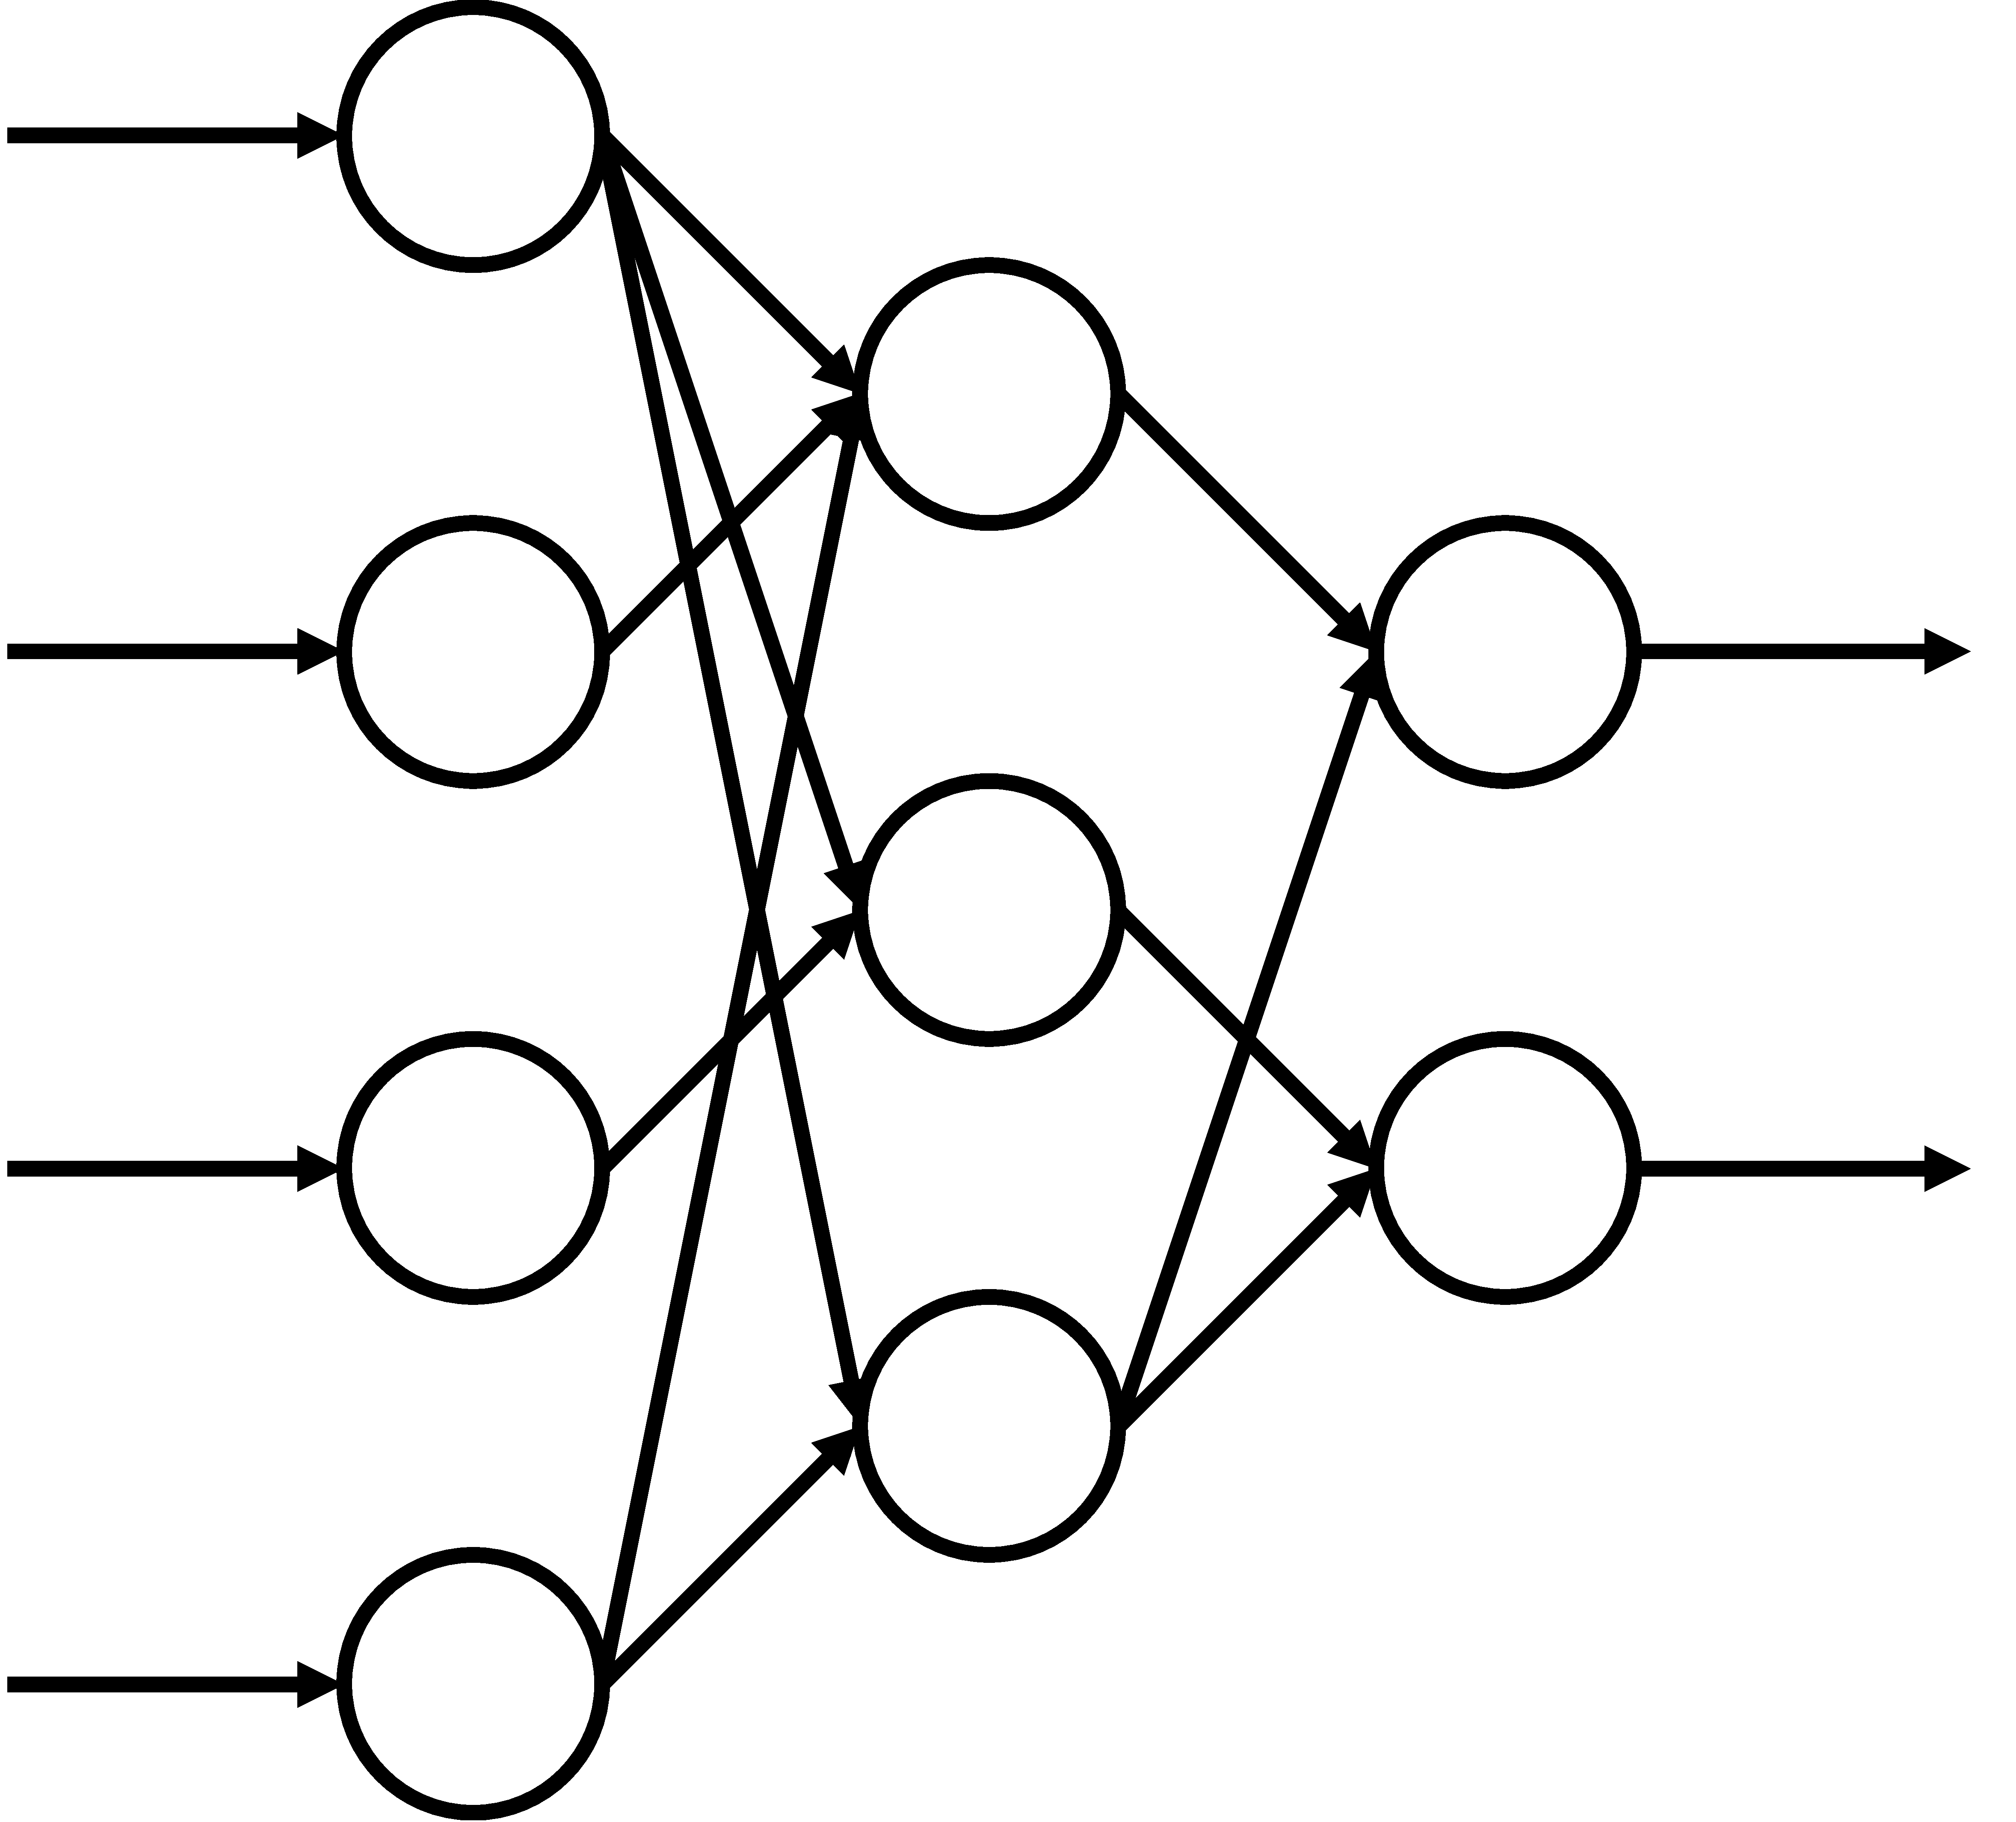
\includegraphics[width=0.75\linewidth]{res/pictures/game-theory-convergence.pdf}
        \captionof{figure}{Konvergenz in der Spieltheorie}
        \label{fig:spieltheorie-konvergenz}
    \end{minipage}
    \hspace*{0.5cm}
    % \hfill
    \begin{minipage}{.385\textwidth}
        \centering
        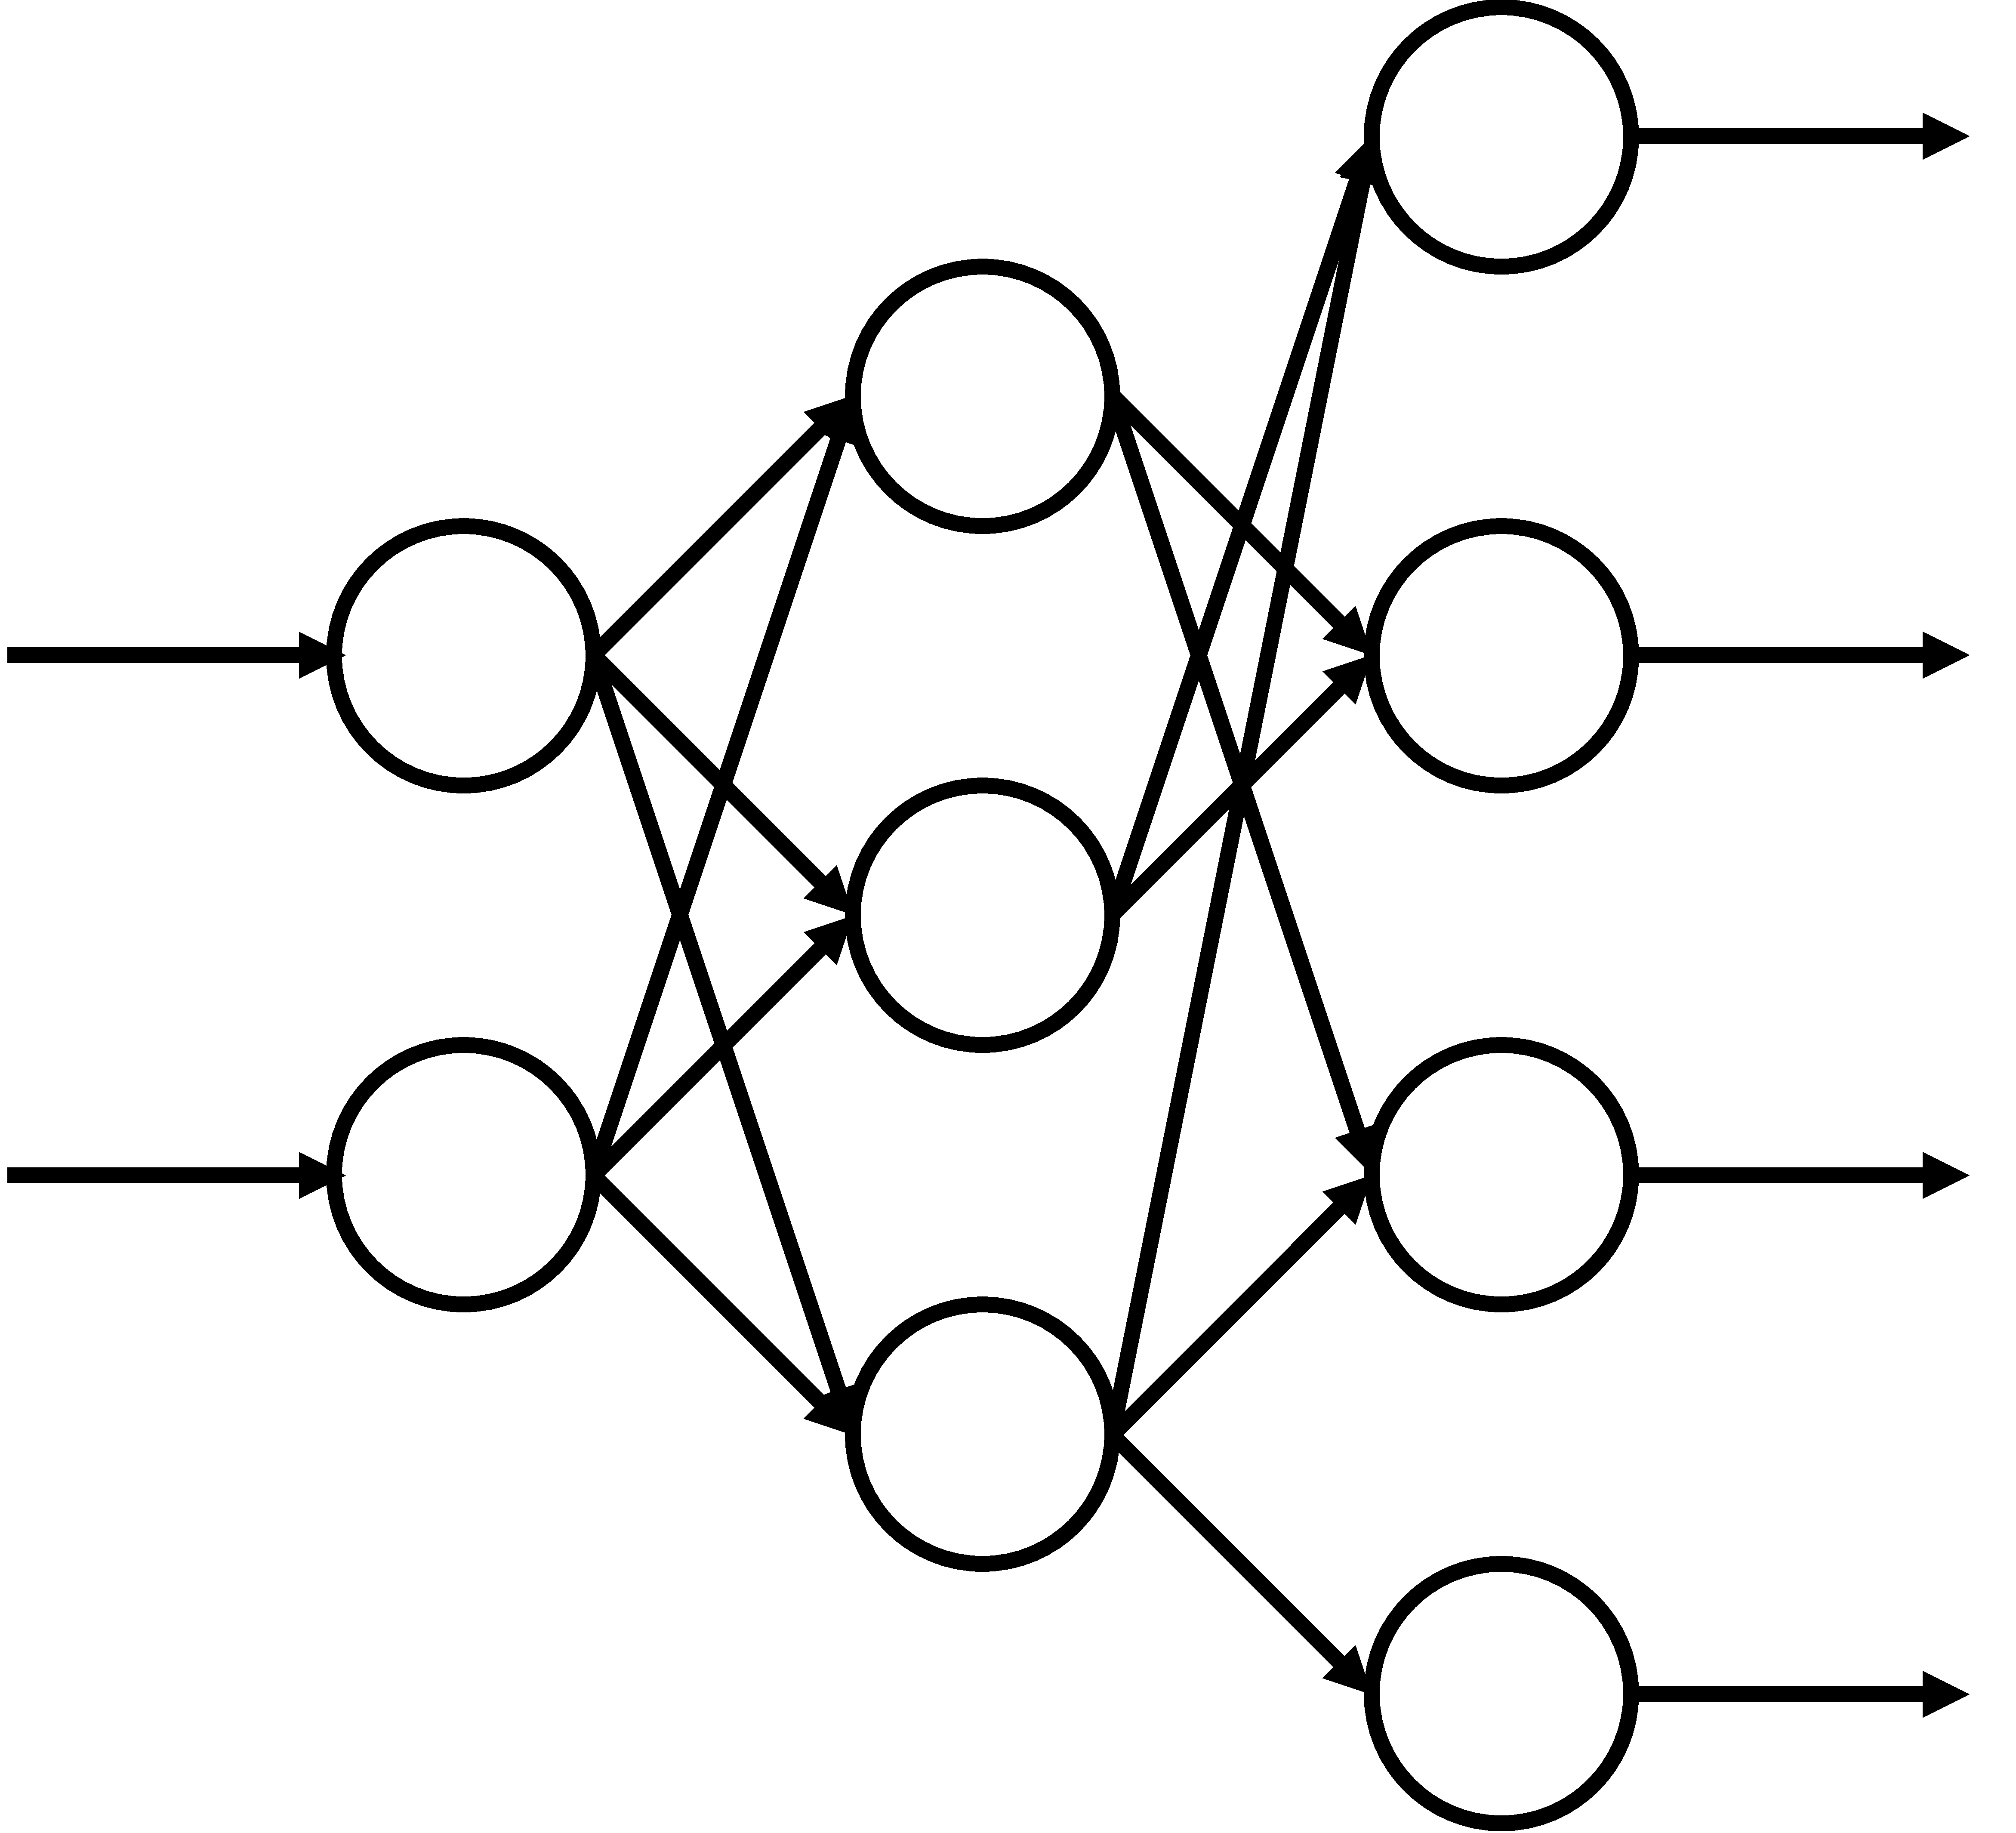
\includegraphics[width=0.75\linewidth]{res/pictures/game-theory-divergence.pdf}
        \captionof{figure}{Divergenz in der Spieltheorie}
        \label{fig:spieltheorie-divergenz}
    \end{minipage}
\end{figure}

\subsection{Spielbaum}

Bei sequenziellen Spielen kann die Struktur des Spiels einschließlich aller Informationen über mögliche Spielverläufe, zeitliche Verläufe der einzelnen Züge der Spieler sowie der Spielzustände zu jedem Zeitpunkt durch einen Spielbaum erfasst werden \cite[S. 13]{2005.SpieltheorieEinführung}.

\begin{wrapfigure}{r}{0.4\textwidth}
    \centering
    % \vspace*{-0.25cm}
    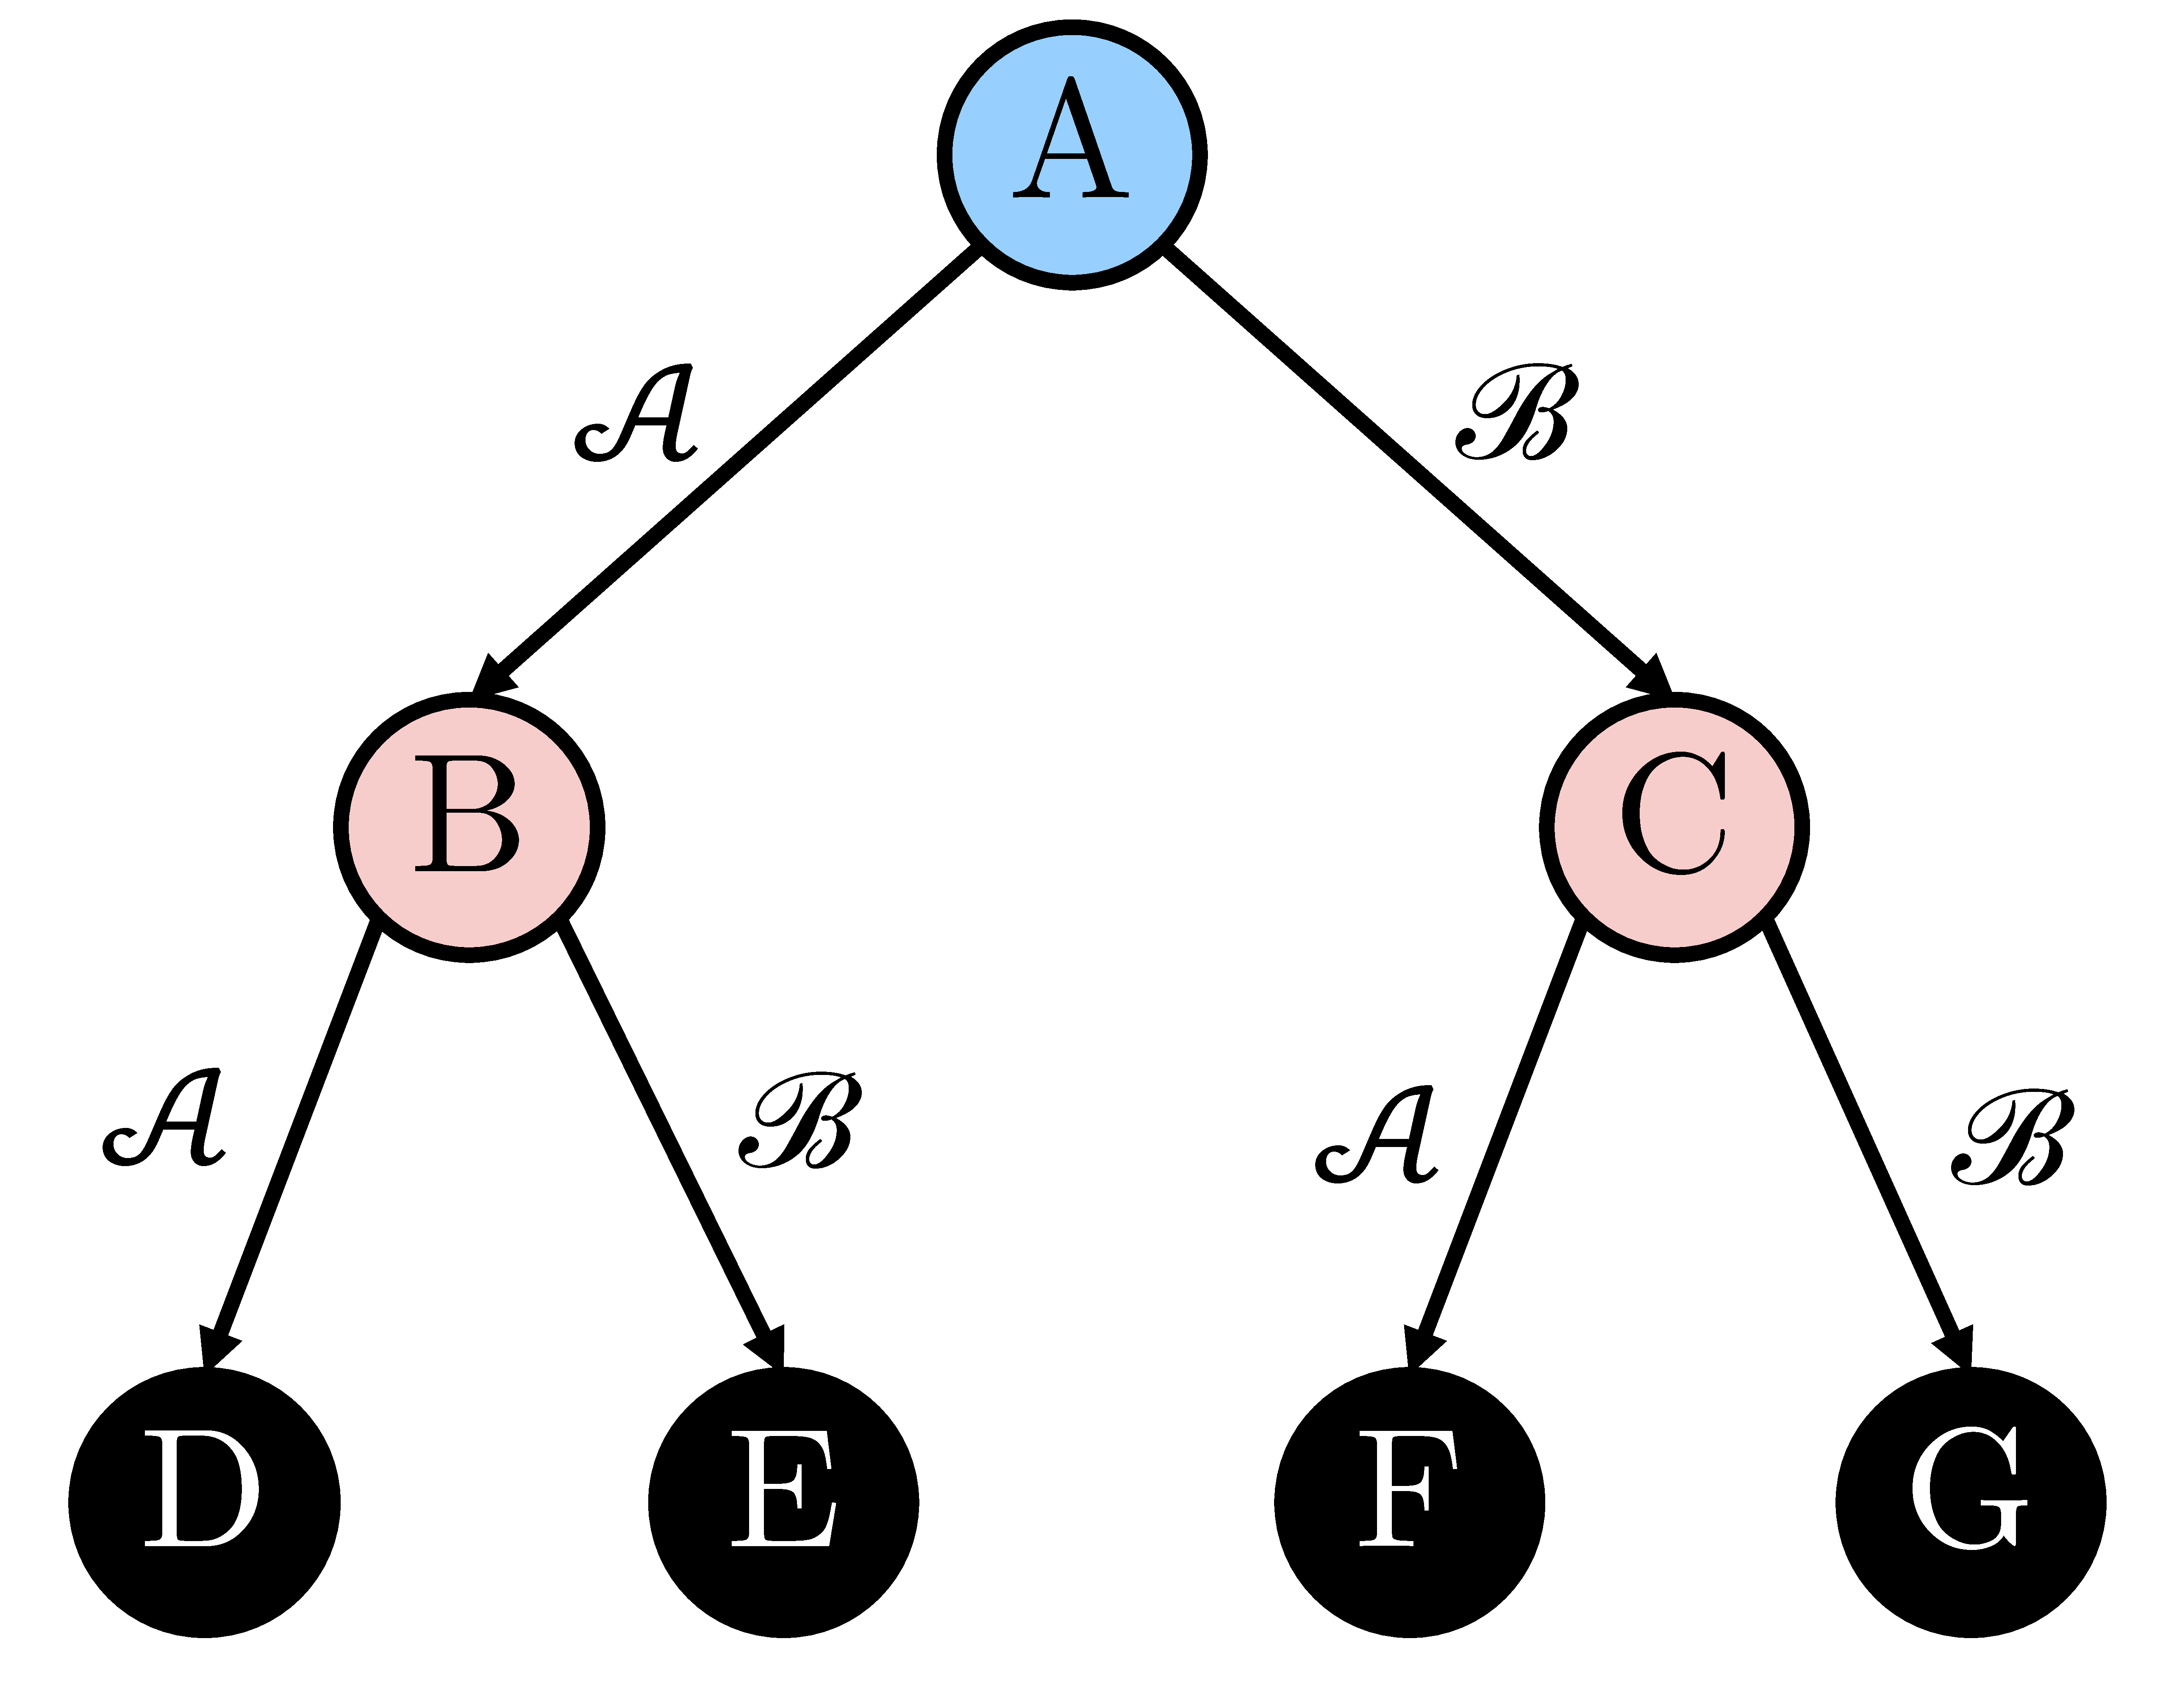
\includegraphics[width=0.37\textwidth]{res/pictures/game-tree.pdf}
    \caption{Spielbaum}
    \label{fig:spielbaum}
    \vspace*{0.5cm}
\end{wrapfigure}

Ein beispielhafter Spielbaum ist in Abbildung \ref{fig:spielbaum} abgebildet. Die einzelnen Knoten des Baums repräsentieren die verschiedenen Zustände des Spiels. Der Wurzelknoten ist der Startzustand. Jedem Knoten ist ein Spieler zugeordnet (in der Abbildung durch die Farbfüllung des Knotens gekennzeichnet). Dieser Spieler kann in dem Zustand aus mehreren Aktionen ($\mathcal{A}$ und $\mathcal{B}$) auswählen, was den Kanten des Baums entspricht. Diese Baumstruktur wiederholt sich, bis das Spiel zu einem Endzustand kommt, welches die schwarz ausgefüllten Knoten in der Abbildung sind. \cite[S. 54]{2014.GameTheoryThroughExamples}

Die Erstellung von Computergegnern basiert in der Regel auf den Spielbäumen. Um optimale Entscheidungen zu treffen, werden verschiedene Spielbaumsuchalgorithmen verwendet, um den Baum zu durchlaufen, verschiedene Positionen zu analysieren und somit die Auswirkungen von Aktionen zu bewerten. Aufgrund der Komplexität vieler Spieler wird dabei oft nur ein Teil des Spielbaums durchsucht, wie beispielsweise bei der »\hyperref[chapter:minimax-algorithmus]{\alpha-\beta-Suche}«, welche den Suchbaum bis zu einer bestimmten Tiefe untersucht. \cite[S. 15]{1194.SearchAndAiInGames}

\subsection{Spielkomplexität}

Die kombinatorische Spieltheorie ist ein Teilbereich der Spieltheorie, der sich mit der Analyse von \emph{zugbasierten} Spielen mit \emph{perfekter Information} befasst. Der Bereich beschäftigt sich mit der Entwicklung verschiedener theoretischer Methoden zur Betrachtung der Spiele. Dazu gehören unter anderem mehrere verschiedene Beschreibungen für die Komplexität von Spielen. Nachfolgend sind drei wesentliche Begriffe für Komplexität in der kombinatorischen Spieltheorie:

\pagebreak

\begin{itemize}
    \item \textbf{Zustandsraum-Komplexität ($\text{\acsp{SSC}}$)}: Die Anzahl der legal erreichbaren Spielpositionen ausgehend von der Ausgangsposition des Spiels. \cite[S. 106]{2007.SolvingGames}
    \item \vspace*{-0.2cm} \textbf{Spielbaumgröße ($\text{\acsp{GTS}}$)}: Die Anzahl der möglichen Spielverläufe ausgehend vom Start des Spiels \cite[S. 1]{2019.GameTreeComplexityEstimation}. Entspricht somit der Anzahl der Blattknoten im Spielbaum.
    \item \vspace*{-0.2cm} \textbf{Spielbaumkomplexität ($\text{\acsp{GTC}}$)}: Diese Komplexität ist definiert als die Anzahl der Blattknoten im Lösungs-Suchbaum des Startzustandes. Der Lösungs-Suchbaum eines Knotens $N$ ist der Spielbaum in voller Breite mit einer Tiefe, die der Lösungstiefe von $N$ entspricht. Die Lösungstiefe von $N$ ist die minimale Tiefe einer ausreichenden Suche mit voller Breite um den spieltheoretischen Wert von $N$ zu bestimmen. \cite[S. 299]{2002.GamesSolved}
\end{itemize}

\vspace*{-0.2cm}
\vspace*{-0.15cm}

\section{Lineare Programmierung}
\label{chapter:lineare-programmierung}

Lineare Programmierung, auch als Lineare Optimierung bezeichnet, ist ein Teilbereich der mathematischen Optimierung, der sich mit der Minimierung oder Maximierung einer Zielfunktion befasst \cite{2024.MathWorksLP}. Besonders ist hierbei, dass sowohl die Zielfunktion als auch alle Nebenbedingungen linear bezüglich der Optimierungsvariable $x$ sind. Lineare Programme werden im Normalfall in der Standardform, die in \ref{eqn:linear-programming} dargestellt ist, angegeben \cite[S. 6]{2023.ConvexOptimization}.

\vspace*{-0.2cm}
\begin{align}
    \label{eqn:linear-programming}
    \minimize_{x}                     & \quad c^\mathsf{T} x                                                                                                    \\
    \text{unter den Nebenbedingungen} & \quad Ax \leq b      & x \in \mathbb{R}^{n}, A \in \mathbb{R}^{m\times n}, b \in \mathbb{R}^{m} \vspace*{-0.2cm} \notag
\end{align}

\begin{wrapfigure}{r}{0.4\textwidth}
    \centering
    \vspace*{-0.75cm}
    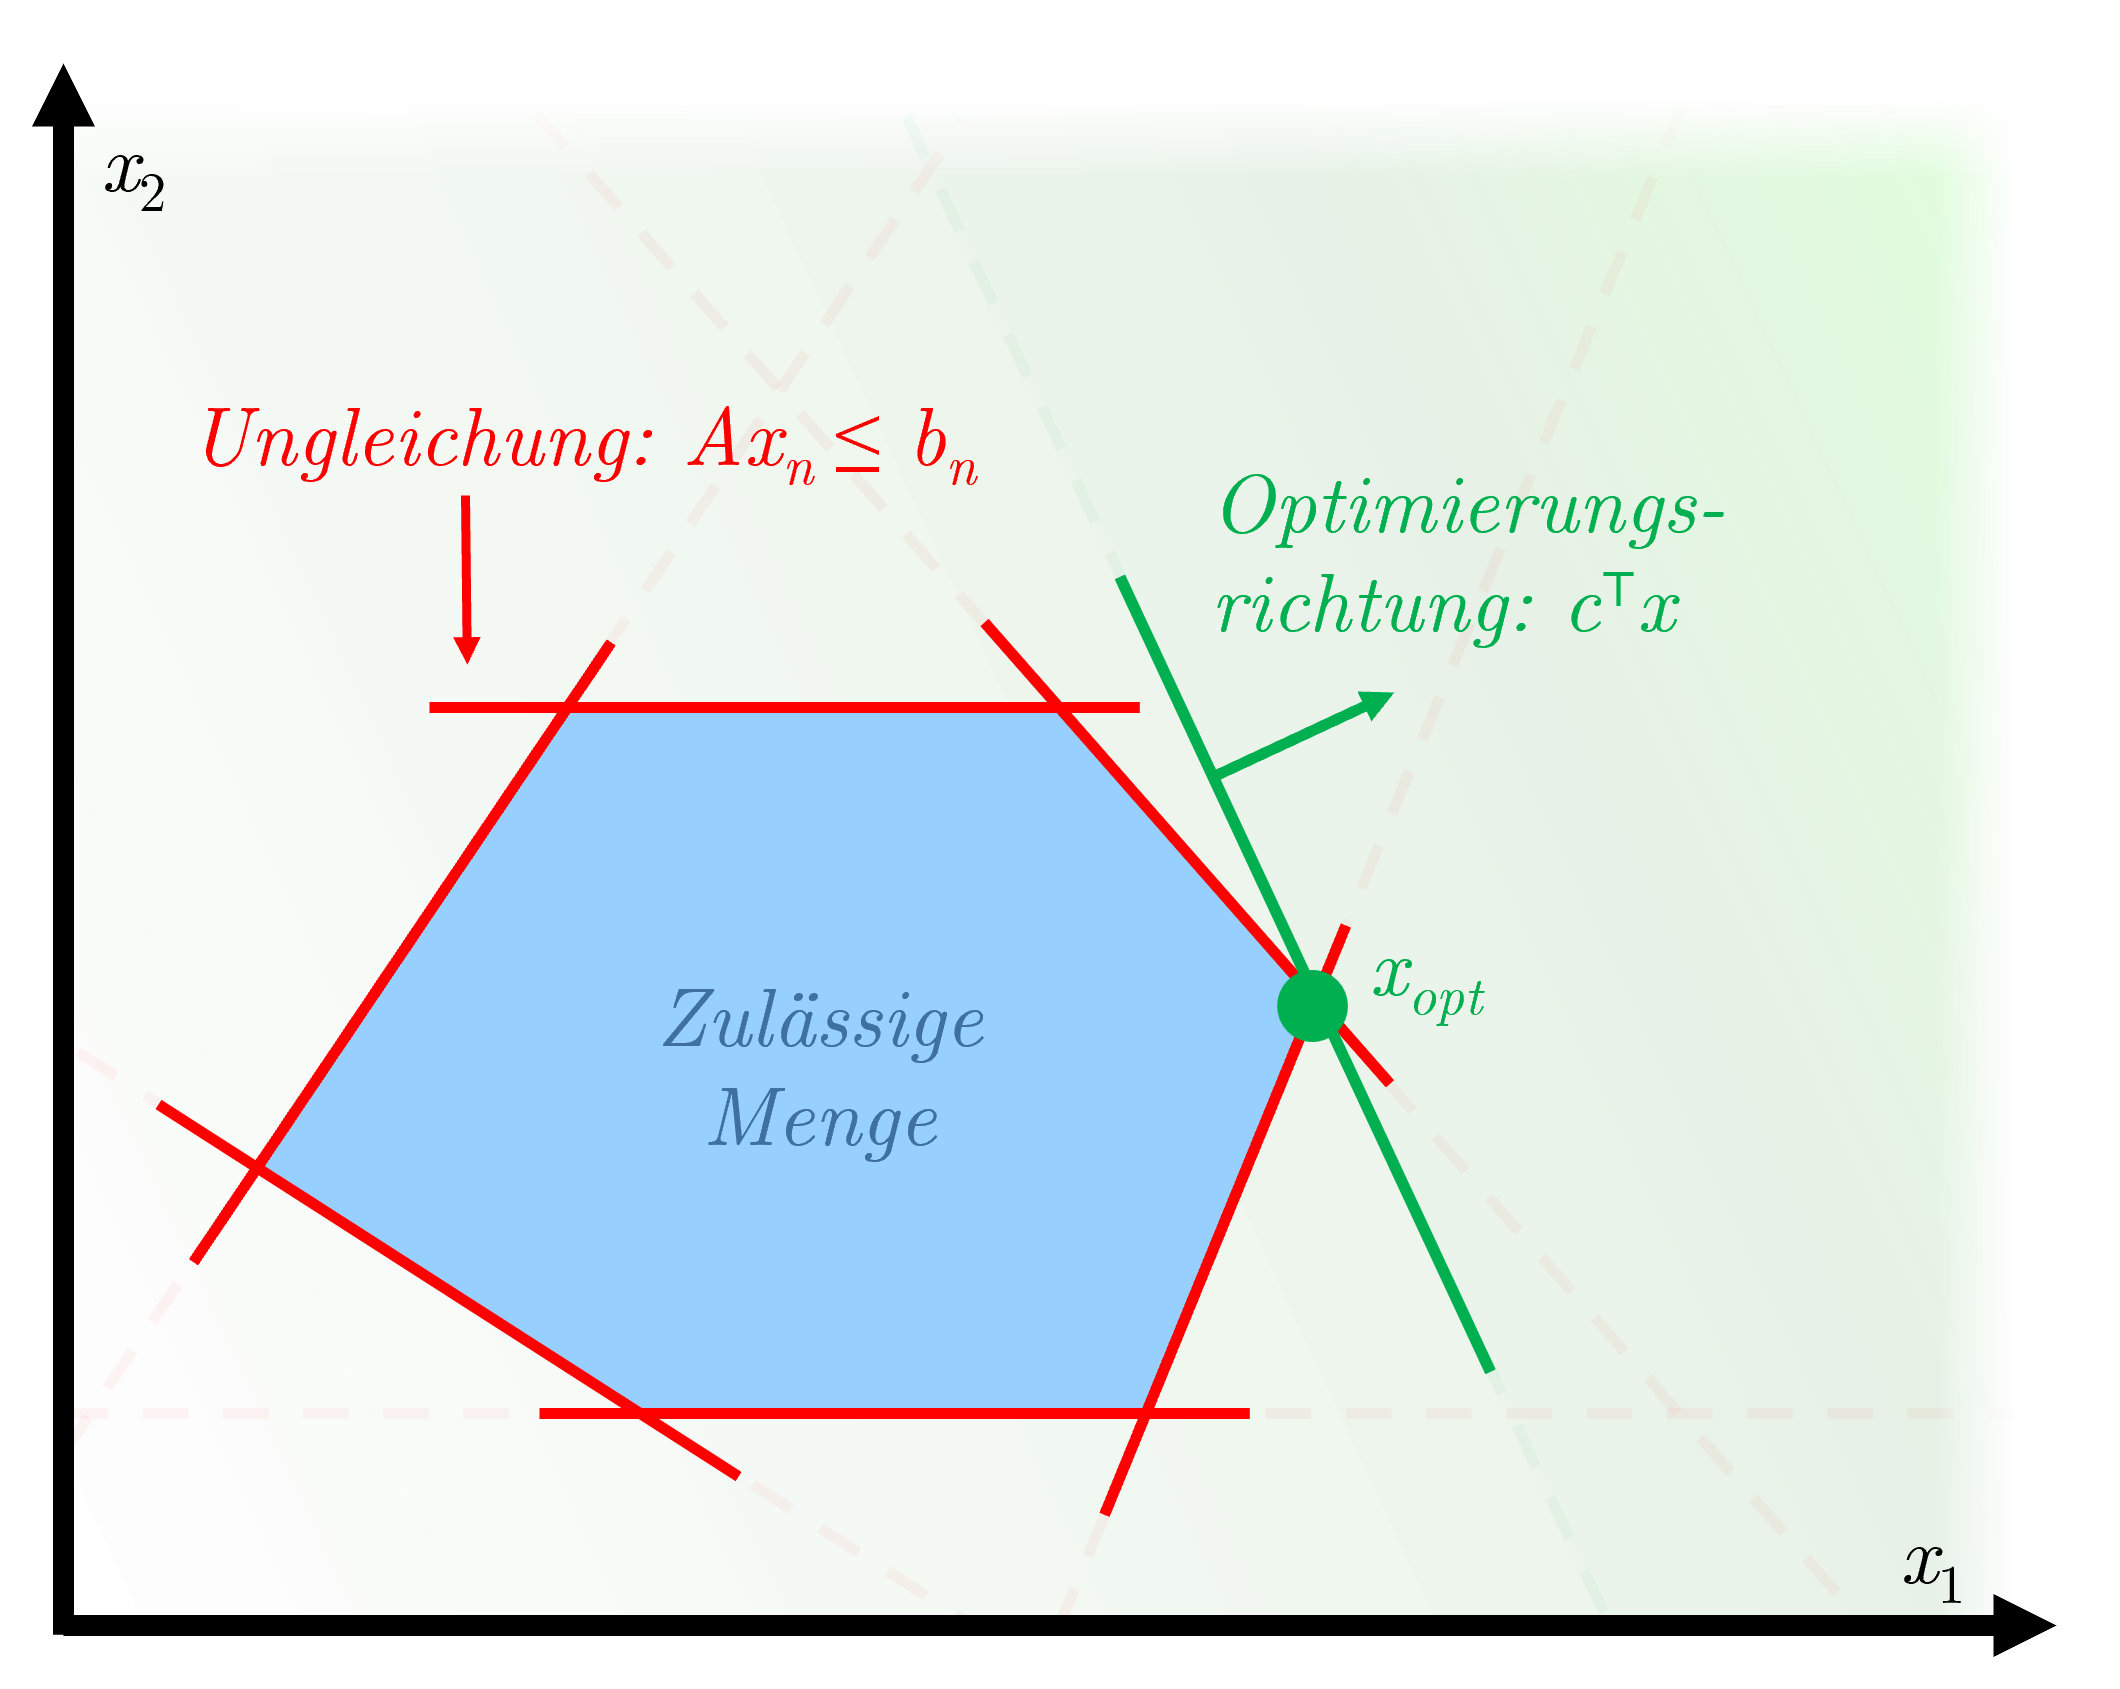
\includegraphics[width=0.38\textwidth]{res/pictures/linear-programming.png}
    \caption[Grafische Lineare Optimierung]{\unskip}
    Grafische Lineare Optimierung
    \label{fig:linear-programming}
    \vspace*{-0.75cm}
\end{wrapfigure}

Grafisch betrachtet ist die lineare Programmierung die Suche in einem zulässigen Suchbereich in Richtung der Zielfunktion. Dieser Suchbereich wird dabei durch die Ungleichungen so eingeschränkt, dass ein Polyeder entsteht \cite[S. 31]{2023.ConvexOptimization}. Dieser grafische Zusammenhang ist in Abbildung \ref{fig:linear-programming} visualisiert. Für lineare Optimierungsprobleme gibt es kein direktes analytisches Lösungsverfahren, jedoch existieren verschiedene Algorithmen, die das Problem in polynomialer Zeit lösen können \cite[S. 6]{2023.ConvexOptimization}.

Die Algorithmen teilen sich dabei in zwei größere Klassen auf:

\begin{itemize}
    \item \emph{Active-Set-Methoden}: Verfahren, bei denen Ungleichungen, die mit Gleichheit gelten, als aktiv betrachtet werden und in das Optimierungsproblem aufgenommen werden \cite[S. 243]{2023.OptimizationLectureNotes}. Solange Ungleichungen strikt gelten, werden sie also in einem Optimierungsschritt nicht betrachtet. Ein Beispiel hierfür ist das Simplex-Verfahren \cite[S. 248]{2023.OptimizationLectureNotes}.
    \item \emph{Innere-Punkt-Verfahren}: Verfahren, bei denen sich der optimalen Lösung vom Innerem des zulässigem Bereichs iterativ angenähert wird. \cite[S. 261]{2023.InteriorPoint}
\end{itemize}

Es gibt verschiedene Programme zur Lösung linearer Optimierungsprobleme. Diese Programme ermöglichen es, das Problem in der oben gezeigten Standardform einzugeben. Das Umformulieren von linearen Optimierungsproblemen in dieser Standardform ist immer möglich und kann oft auch automatisch übernommen werden, wie beispielsweise mit der Python-Bibliothek CVXPY \cite[S. 1]{2016.CVXPY}.

Eine Variation von Linearer Programmierung ist \ac{ILP}, bei dem gefordert wird, dass es sich bei den Optimierungsvariablen $x$ um ganze Zahlen $\mathbb{Z}^{n}$ handelt. Im Gegensatz zum ursprünglichem Problem ist \ac{ILP} NP-vollständig, was das Erstellen effizienter Algorithmen erschwert \cite[S. 173]{2002.MathProgramming}. Lineare Optimierungsprobleme mit sowohl kontinuierlichen als auch diskreten ganzzahligen Variablen werden als \ac{MILP} bezeichnet.

\section{Minimax-Algorithmus}
\label{chapter:minimax-algorithmus}

Suchalgorithmen beachten jede derzeit zur Verfügung stehende Aktion, anschließend jede Aktion, die auf die vorherige Aktion folgen kann und immer so weiter. Das Ziel eines solchen Suchalgorithmus ist das Finden von Endzuständen, welche die vorher gegebenen Zielkonditionen erfüllen. Wird ein solcher Zustand gefunden, so sind die Aktionen bekannt, welche zum Erreichen des Zielzustands passieren werden müssen. In einem kompetitiven Spiel, bei dem ein Gegner beteiligt ist und ein anderes, reziprokes Ziel als der Spieler hat, kann selbst bei Findung eines Zielzustandes nicht davon ausgegangen werden, dass der Gegner die zum Ziel führenden benötigten Aktionen nicht tätigt.

In einem klassischen Spiel mit Sieg, Unentschieden und Niederlage ist es das Ziel des Gegners den Spielzustand in Richtung seines Sieges zu lenken oder ein Unentschieden zu lenken, keinesfalls jedoch in den Zielzustand des Spielers. Suchalgorithmen können in diesen Fall allerdings auch Lösungen finden, sie müssen nur um Taktiken erweitert werden, um die Aktionen des Gegners mitzubeachten. \cite{AlgorithmsMinimax}

Für Spiele mit zwei Spielern ist der Minimax-Algorithmus eine solche Taktik, welcher den Fakt ausnutzt, dass die zwei Spieler genau gegensätzliche Ziele haben, wodurch der Algorithmus dann Voraussagungen über zukünftige Spielstände macht und die Gewinnchancen für einen Spieler optimiert. Die Theorie hinter dem Algorithmus besagt, dass der Gegner versuchen wird den Wert zu minimieren, welchen der Algorithmus maximieren will. Daraus lässt sich schließen, dass der Algorithmus immer den die Aktion oder Pfad im Spielbaum nehmen sollte, bei dem der Gegner die geringste Minimierung bewirken kann. In einem idealen Fall kann der Algorithmus mit beliebig viel Speicherplatz und beliebig viel Zeit alle Endzustände des Spiels und somit den gesamten Spielbaum berechnen, um anschließend von unten nach oben den gewinnbringenden Pfad zu finden. \cite{AlgorithmsMinimax}

\begin{figure}[!ht]
    \centering
    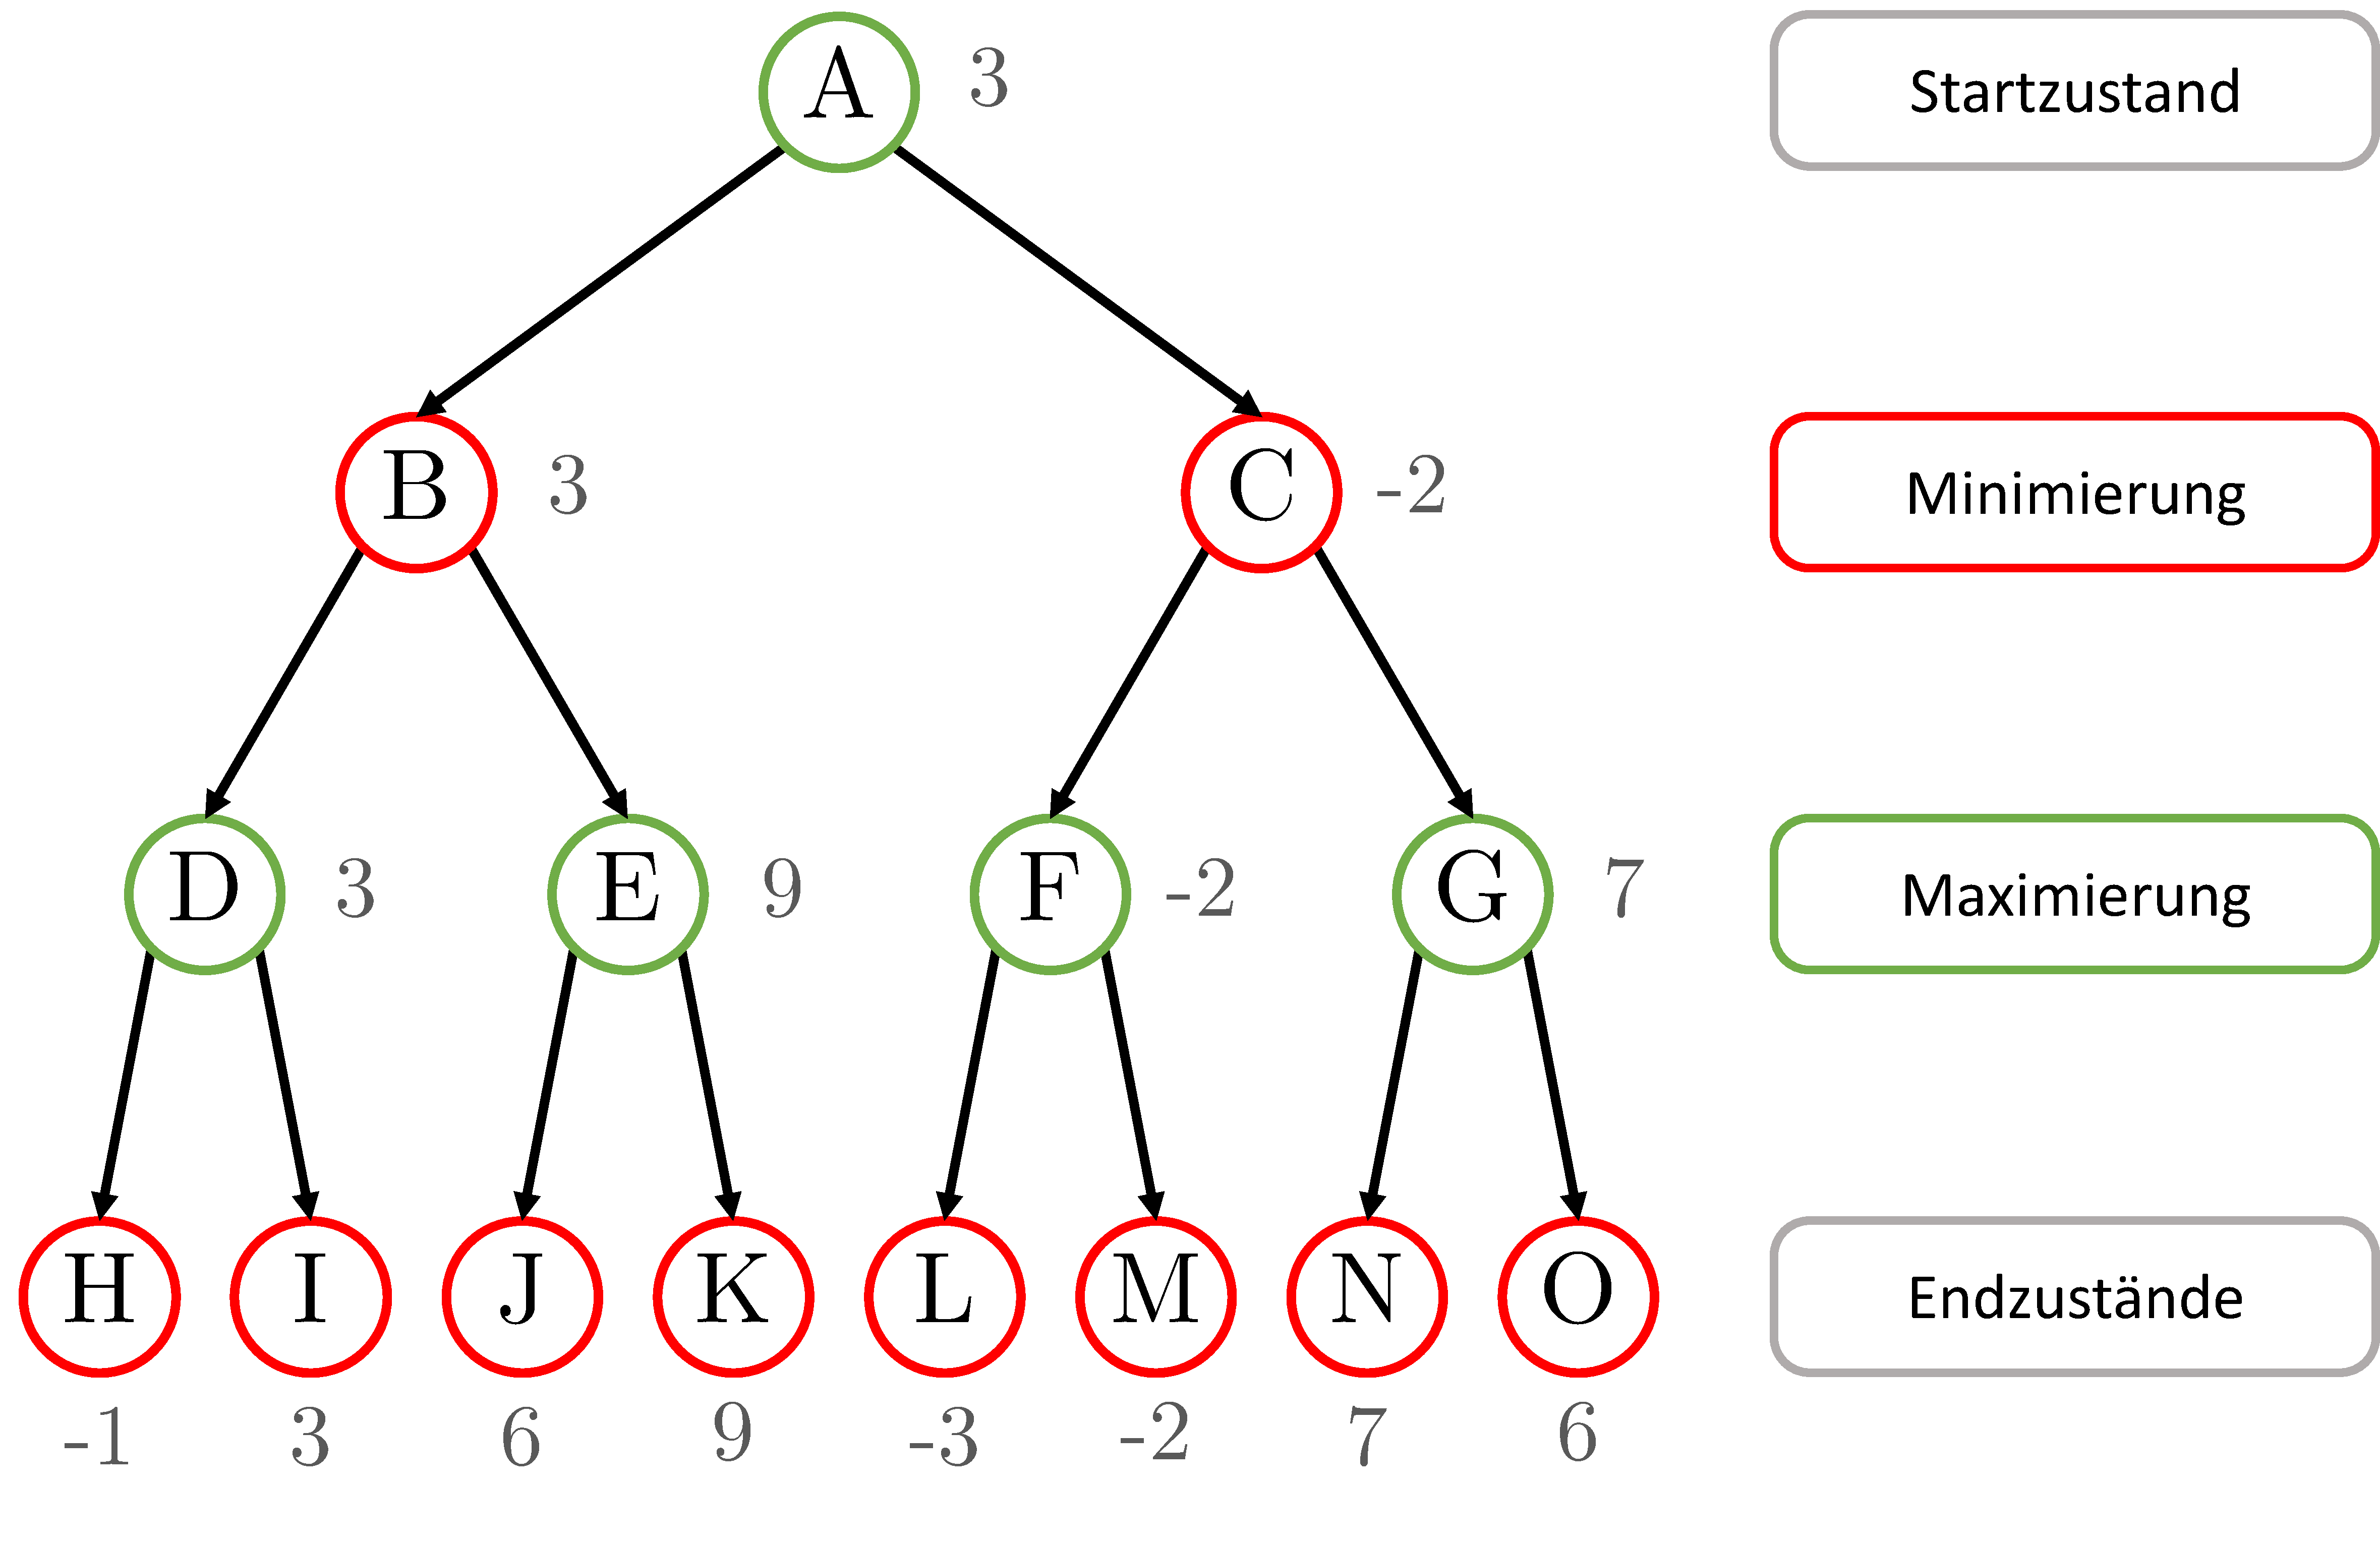
\includegraphics[width=\textwidth]{res/pictures/minimax-tree.pdf}
    \caption{Spielbaum von Minimax-Algorithmus}
    \label{fig:minimax-tree}
\end{figure}

In der Abbildung \ref{fig:minimax-tree} ist ein Spielbaum eines Spiels zwischen dem Minimax-Algorithmus und dem Gegner abgebildet. Das Ziel des Algorithmus ist am Ende des Spiels eine möglichst hohe Zahl zu erreichen, während der Gegner eine möglichst geringe Zahl erreichen will. Der Algorithmus startet mit seiner Evaluierung des Baums unten bei den Endzustandsknoten H und I. Der darüber liegende Knoten D ist ein Knoten einer Maximierungsstufe, da der Algorithmus hier den weiteren Spielverlauf durch seine Auswahl des folgenden Knoten bestimmen kann. Hier muss demnach der größte Wert ausgewählt werden, damit der Algorithmus den Pfad für den eigenen Sieg finden kann. Der ausgewählte Wert wird für den Maximierungsknoten D übernommen. Anschließend werden die Knoten J und K verglichen und der größere Wert 9 im Maximierungsknoten E gespeichert. Jetzt liegen beiden benötigten Werte für den die Evaluierung des Knoten B vor. Da allerdings der Gegner hier am Spielzug ist und sein Ziel eine möglichst kleine Zahl ist, wird der minimale Wert von den Knoten D und E gesucht. Dementsprechend wird in den Minimierungsknoten B der Wert 3 gespeichert. Die Minimierungs- und Maximierungsschichten wiederholen sich immer abwechselnd im Spielbaum, da die beiden Spieler jeweils abwechselnd ihre Spielzüge ziehen können. Im Startzustandsknoten ist folglich der Minimax-Algorithmus am Zug, der bereits die eine Hälfte des Spielbaums evaluiert hat und dem Algorithmus eine Endwertung von 3 sichert, wenn der Gegner jeweils seine besten Züge macht. Die Evaluierung der zweiten Hälfte des Spielbaums und des Knotens C passiert auf gleiche Weise wie zuvor. Nun liegt fast der gesamte Spielbaum vor und der Algorithmus kann seinen Startzug bestimmen. Dadurch befindet sich der Spielzustand in einer Maximierungsschicht, weshalb von den Knoten B und C, der Knoten B mit dem höheren Wert 3 ausgewählt wird. Das Spiel wird demnach voraussichtlich die Knoten A, B, D durchlaufen und mit dem Knoten I enden.

Ein Problem des normale Minimax-Algorithmus ist leicht erkannt: Der Algorithmus kann bei nicht-trivialen Spielen auf Grund von Zeit- und oder Speicherbeschränkungen nicht bis zu den Endzuständen des Spielbaums vordringen und kann somit keine Zwischenknoten und optimale Spielpfade evaluieren. Abhilfe schaffen in diesem Fall Heuristiken, welche den Spielzustand der künstlich gewählten Zwischenknoten abschätzen, wobei der Erfolg dieses Algorithmus dann hauptsächlich von der Korrektheit der Heuristiken abhängig ist. \cite{AlgorithmsMinimax}

\subsection{Alpha-Beta-Pruning}

Alpha-Beta-Pruning ist eine Optimierung für den Minimax-Algorithmus, um die Anzahl an zu evaluierenden Knoten des Spielbaums zu minimieren. Die Bestimmung der korrekten Algorithmus-Entscheidung kann nämlich auch ohne die Evaluierung von jedem Knoten im Spielbaum bestimmt werden, indem die Optimierung nur Spielbaumzweige eliminiert, die keinen Einfluss auf die Entscheidung des Minimax-Algorithmus haben. \cite{AlgorithmsAlphaBetaPruning}

Der Minimax-Algorithmus, im Anhang Algorithmus \ref{algo:minimax}, wird für die optimierte Variante mit Alpha-Beta-Pruning um die zwei namensgebenden Eingabeparameter $\alpha$ und $\beta$ erweitert und ist unter Algorithmus \ref{algo:minimax-alpha-beta} zu sehen. Wie der Standardalorithmus läuft die Variante mit Alpha-Beta-Pruning mit rekusiver Tiefensuche durch den Spielbaum und berechnet im Anschluss den optimalen Weg für einen Spieler.

\refstepcounter{lstlisting}
\addcontentsline{lol}{lstlisting}{\protect\numberline{\thelstlisting}Pseudocode vom Minimax-Algorithmus mit Alpha-Beta-Pruning}

\begin{algorithm}
    \caption{Pseudocode vom Minimax-Algorithmus mit Alpha-Beta-Pruning}
    \label{algo:minimax-alpha-beta}
    \begin{algorithmic}[1]
        \Function{alphabeta}{node $n, \alpha, \beta$}
        \If{$n$ is a terminal node}
        \State \Return value of $n$
        \ElsIf{$n$ is a maximizer node}
        \For{each child node $c$ of $n$}
        \State $value \gets$ \Call{alphabeta}{$c, \alpha, \beta$}
        \State $\alpha \gets \max(\alpha, value)$
        \If{$\alpha \geq \beta$}
        \State \textbf{break}
        \EndIf
        \EndFor
        \State \Return $\alpha$
        \ElsIf{$n$ is a minimizer node}
        \For{each child node $c$ of $n$}
        \State $value \gets$ \Call{alphabeta}{$c, \alpha, \beta$}
        \State $\beta \gets \min(\beta, value)$
        \If{$\beta \leq \alpha$}
        \State \textbf{break}
        \EndIf
        \EndFor
        \State \Return $\beta$
        \EndIf
        \EndFunction
    \end{algorithmic}
\end{algorithm}

Die Eingabeparameter sind der Startknoten $n$, $\alpha$, welcher der beste Wert ist, den der maximierende Spieler bisher erreicht hat und $\beta$, welcher der beste Wert ist, den der minimierende Spieler bisher erreicht hat. Beim ersten Aufruf müssen die Werte $\alpha$ auf $-\infty$ und $\beta$ auf $+\infty$ gesetzt werden, was die jeweils schlechtesten Werte für die Spieler sind, damit jeder bessere Wert gewertet wird. Der Minimax-Algorithmus mit Alpha-Beta-Pruning funktionert wie folgt:

\begin{enumerate}
    \item Wenn der Knoten $n$ ein Endknoten ist, wird der Wert dieses Knotens zurückgegeben
    \item Wenn der Knoten $n$ ein Maximierungsknoten ist, werden alle Kinderknoten durchlaufen, um den besten Zug zu finden.
          \begin{enumerate}
              \item Bestimmung des Wertes des Kindknotens $c$ durch rekursiven Selbstaufruf
              \item Aktualisierung von $\alpha$, falls der Wert von $c$ größer ist.
              \item Falls $\alpha \geq \beta$ ist, wird das Durchlaufen der Kinderknoten abgebrochen, da der Gegner einen besseren Zug durch andere Pfadwahl nicht zulassen würde.
              \item Zurückgeben von $\alpha$, was der maximale Endwert bei optimaler Spielablauf von $n$ ist.
          \end{enumerate}
    \item Wenn der Knoten $n$ ein Minimierungsknoten ist, werden alle Kinderknoten durchlaufen, um den besten Zug für den Gegner zu finden.
          \begin{enumerate}
              \item Bestimmung des Wertes des Kindknotens $c$ durch rekursiven Selbstaufruf
              \item Aktualisierung von $\beta$, falls der Wert von $c$ kleiner ist.
              \item Falls $\beta \leq \alpha$ ist, wird das Durchlaufen der Kinderknoten abgebrochen, da kein besserer Zug für den Gegner möglich ist, als der Zug, welcher schon vom maximierenden Spieler  gefunden wurde.
              \item Zurückgeben von $\beta$, was der minimale Endwert bei optimalem Spielablauf von $n$ ist.
          \end{enumerate}
\end{enumerate}

\begin{figure}[!ht]
    \centering
    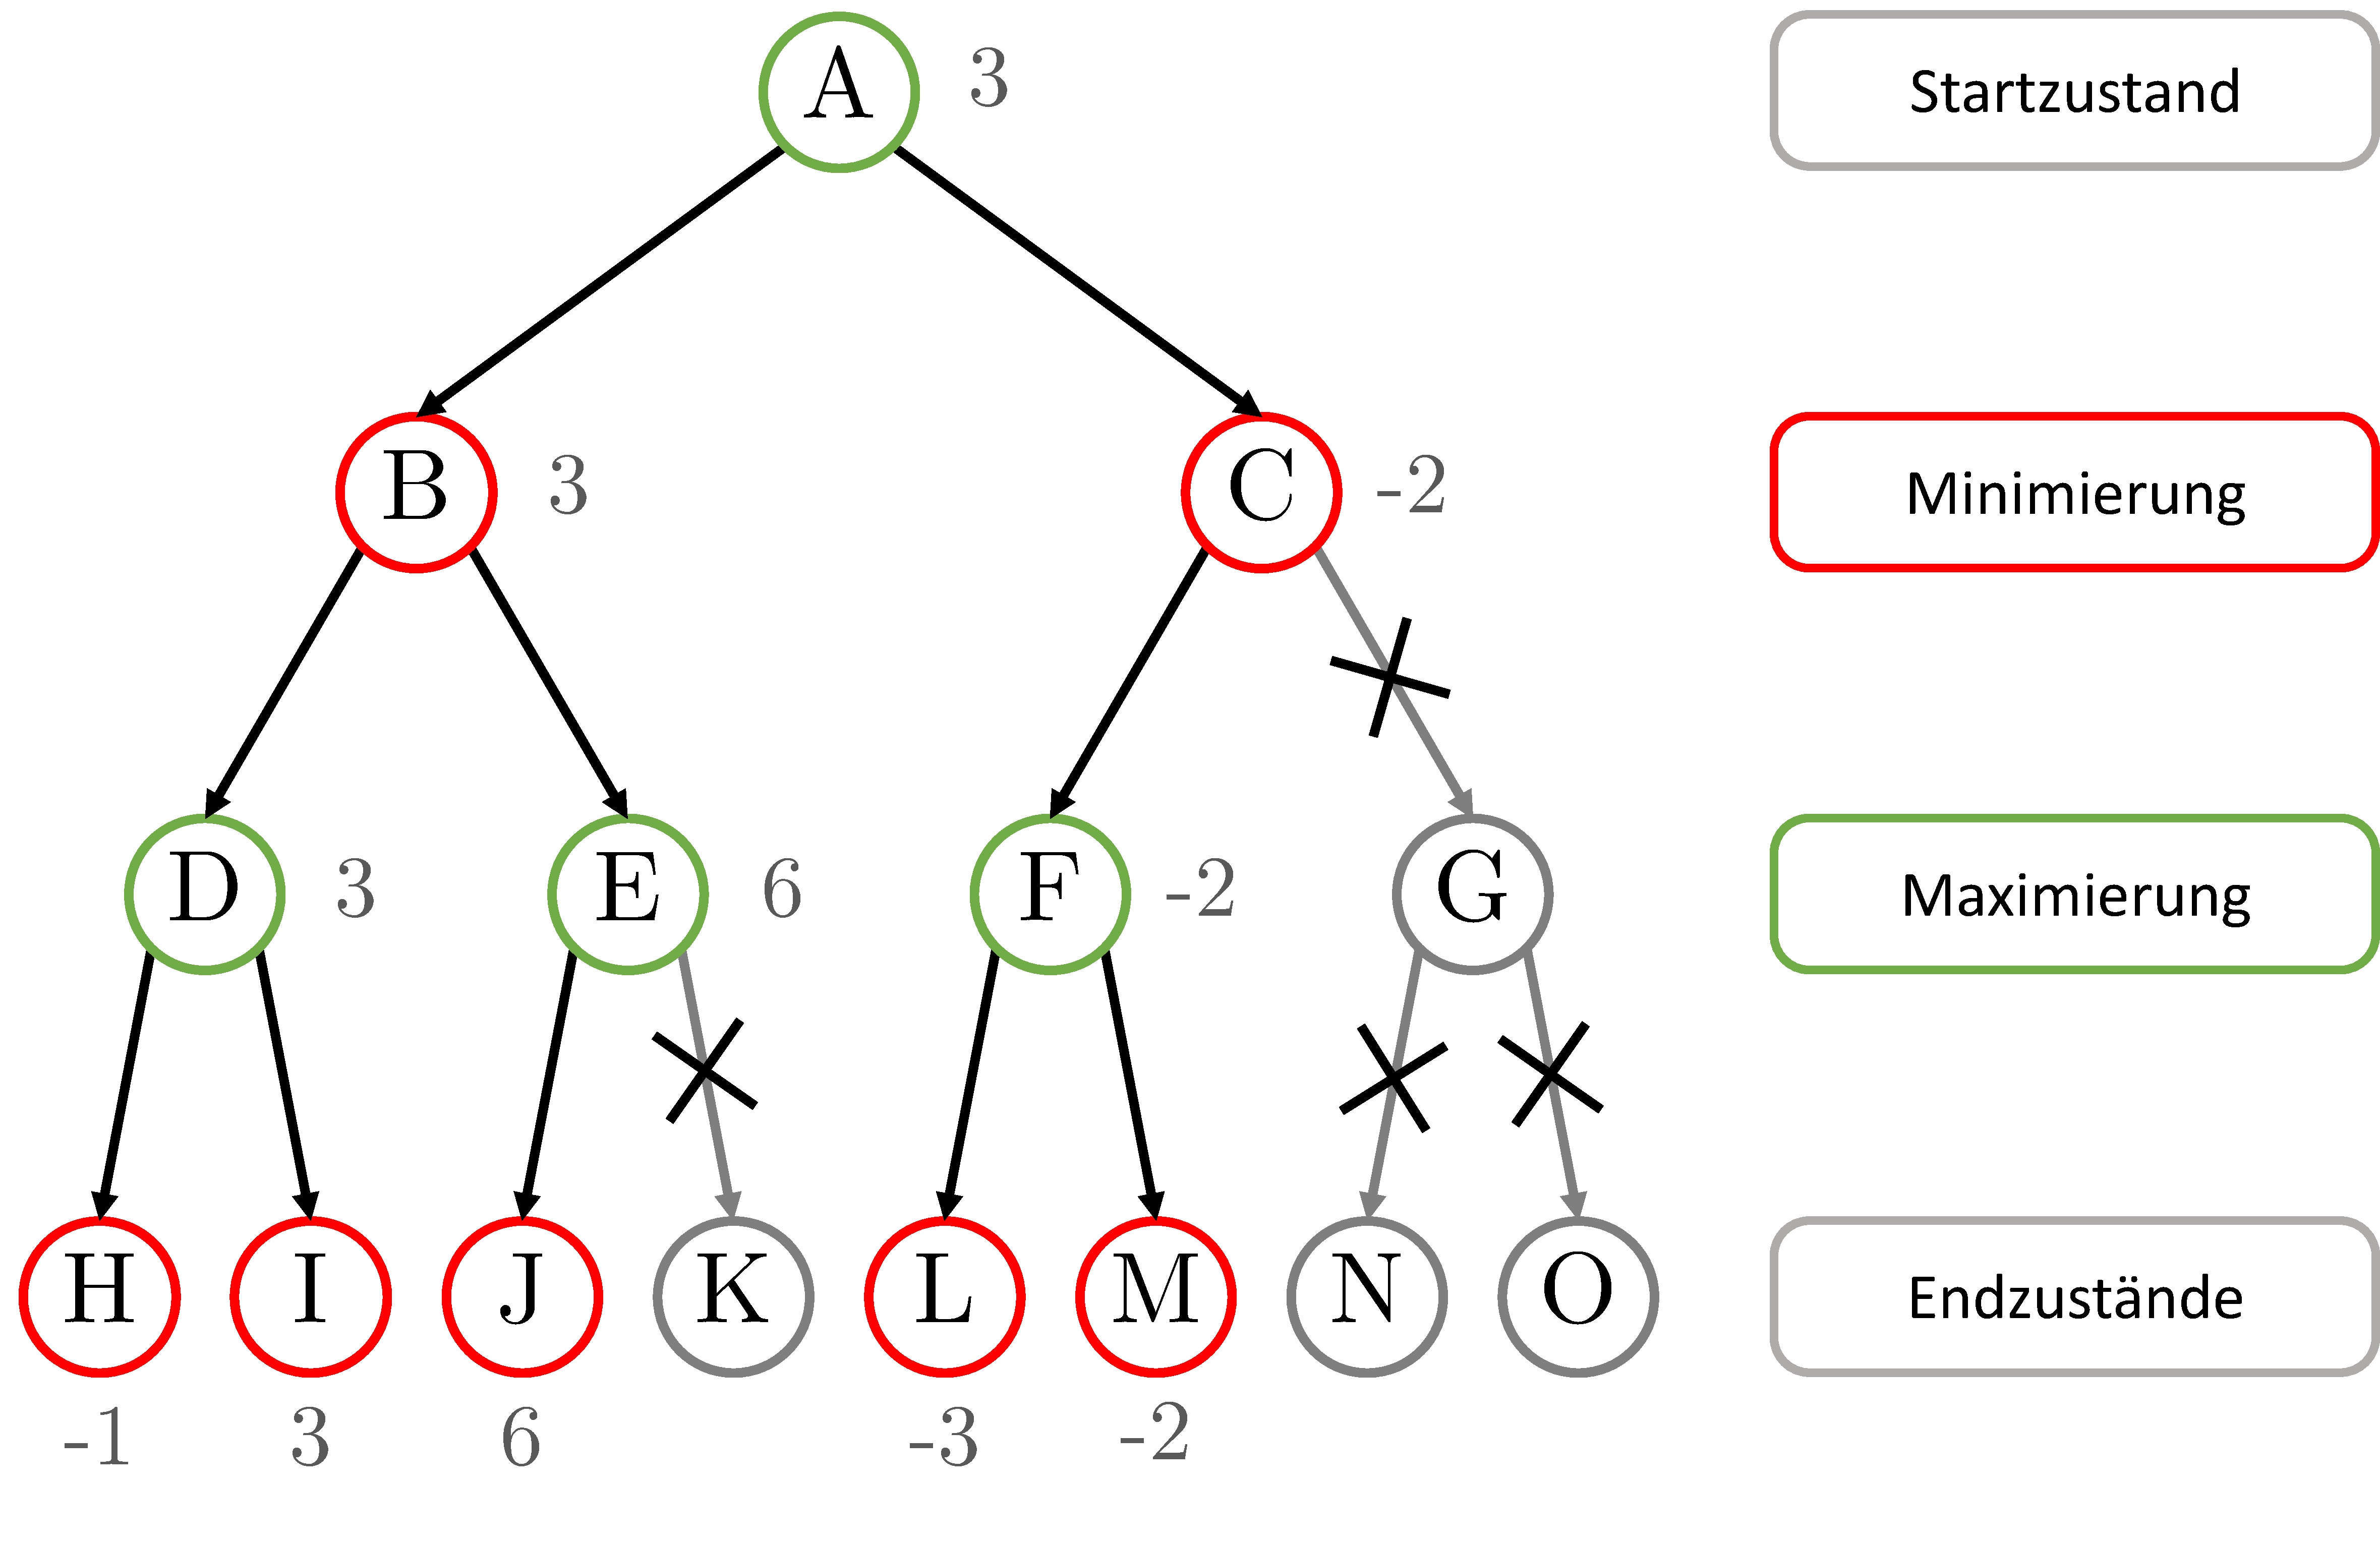
\includegraphics[width=\textwidth]{res/pictures/minimax-tree-with-a-b-pruning.pdf}
    \caption{Spielbaum von Minimax-Algorithmus mit Alpha-Beta-Pruning}
    \label{fig:minimax-a-b-tree}
\end{figure}

Wenn mit dieser optimierten Variante des Minimax-Algorithmus das gleiche, vorher abgebildete Spiel nocheinmal wiederholt wird, ist der Spielbaum kleiner, in Abbildung \ref{fig:minimax-a-b-tree} zu sehen, aber der optimale Spielablauf der Knoten A, B, D und I wird trotzdem gefunden. Am Maximierungsknoten E muss der zweite Kindknoten K nicht evaluiert werden, da am Minimierungsknoten B der Kindknoten D mit Wert 3 ausgewählt wird, weil der Kindknoten E den höheren Wert 6, bei Auswahl von Auswahl von J annehmen könnte. Am Minimierungsknoten C muss der zweite Kindknoten G und die folgenden Knoten nicht evaluiert werden, da dem Maximierungsknoten A im Vergleich zum geringen Wert $-2$ von C schon der höhere Wert 3 von Knoten B zur Auswahl steht. In beiden Fällen kann ein \enquote{Pruning}, dt. Beschneidung, der Zweige des Spielbaum ohne Einfluss auf die Suche nach dem optimalen Spielverlauf stattfinden. Im schlechtesten Fall sind die Zweige nach Werten aufsteigend sortiert, sodass der Algorithmus wie der Minimax-Algorithmus handelt und eine Laufzeitkomplexität von $\mathcal{O}(w^{d})$. $w$ bezeichnet den durchschnittlichen Verzweigungsfaktor und $d$ die Tiefe des Spielbaums, wobei der Verzweigungsfaktor beschreibt die maximale Anzahl an Kindknoten eines Knoten. Im besten Fall sind die Spielzüge absteigend geordnet, also genau umgekehrt zum schlechtesten Fall, wodurch der erste evaluierte Kindknoten den besten Wert liefert und die Laufzeitkomplexität innerhalb von $\mathcal{O}\left(w^{\lfloor d/2\rfloor}\right)$ liegt. Für den durchschnittlichen Fall ergibt sich eine Komplexität von $\mathcal{O}\left(w^{3d/4}\right)$, was besonders bei umfangreichen Berechnungen diesem Algorithmus einen signifikanten Vorteil bringt. \cite[S. 3 ff.]{2017.AlphaBeta}

\section{Monte Carlo Tree Search}
\label{chapter:monte-carlo-tree-search}

\acf{MCTS} ist ein Suchalgorithmus, welcher verwendet wird, um in einem Spiel die beste Aktion zu finden. Dazu wird der Algorithmus während der Entscheidungszeit des Computerspielers ausgeführt. Innerhalb dieser Zeit wird schrittweise ein Suchbaum erstellt. Dabei wird für jede Aktion eine Heuristik erstellt, indem sehr viele Spiele zufällig bis zum Ende ausgespielt werden. Dadurch ergibt sich über die Zeit eine Wahrscheinlichkeit für das Ergebnis des Spiels für jede mögliche Aktion \cite[S. 61]{2008.ParallelMCTS}. Der \ac{MCTS}-Suchprozess besteht aus vier Phasen:

\begin{enumerate}
    \item \textbf{Selektion}: Der Suchbaum wird beginnend ab dem Wurzelknoten bis zu einem Blattknoten durchlaufen, indem in jeder Ebene immer genau ein Kindknoten nach einer bestimmten Richtlinie ausgewählt wird. \cite[S. 187]{2018.ReinforcementLearning}
    \item \textbf{Expansion}: Der ausgewählte Blattknoten wird um ein weiteres Kind erweitert, indem ein noch nicht erforschte Aktion ausgeführt wird. \cite[S. 61]{2008.ParallelMCTS}
    \item \textbf{Simulation}: Ausgehend vom neu hinzugefügten Knoten wird das Spiel bis zum Ende simuliert, indem bis Spielende zufällige Aktionen ausgeführt werden. \cite[S. 61]{2008.ParallelMCTS}
    \item \textbf{Backpropagation}: Das Ergebnis der Simulation wird durch den Suchbaum rückpropagiert, indem das Ergebnis (Gewonnen oder Verloren) ausgehend von dem in Zweitens neu hinzugefügten Knoten bis zum Wurzelknoten hochgereicht wird. \cite[S. 187]{2018.ReinforcementLearning}
\end{enumerate}

Die vier Phasen sind anschaulich in Abbildung \ref{fig:mcts-phases} dargestellt. Diese Phasen werden so lange wiederholt, bis die Entscheidungszeit vorbei ist.

\begin{figure}[!ht]
    \centering
    
\includegraphics[width=\textwidth]{res/pictures/mcts-phases.pdf}
    \caption{Phasen des \acs{MCTS} Algorithmus}
    \label{fig:mcts-phases}
\end{figure}

Für die erste Phase der Selektion wird im Normalfall die in \ref{eqn:uct} dargestellte \ac{UCT} Formel verwendet. Die \ac{UCT} Formel balanciert die Entscheidung zwischen der Ausnutzung von bereits bekannten Aktionen mit der Erkundung von unsicheren Aktionen \cite[S. 206]{2009.ComputerGoMCTS}. Dazu wird im ersten Teil die Anzahl der Siege ($w$) durch die Anzahl der Besuche des Kindknotens ($n$) geteilt. Dieser Term wird immer größer, je öfters eine Simulation nach einem Knotenbesuch gewonnen wird. Der andere Term wird immer größer, je weniger ein Knoten im Vergleich zu seinem Elternknoten ($N$) besucht wird und erzwingt somit auch die Erkundung weniger besuchter Knoten. Bei $c$ handelt es sich um eine Erkundungskonstante, welche das Verhältnis zwischen Ausnutzung und Exploration regelt und normalerweise auf $\sqrt{2}$ gesetzt wird.

\begin{equation}
    \label{eqn:uct}
    \mathbb{U}\mathbb{C}\mathbb{T} = \frac{w}{n} + c \cdot \sqrt{\frac{\ln N}{n}}
\end{equation}

Ein entscheidender Vorteil von \ac{MCTS} ist, dass keine statische Evaluierungsfunktion einer Position wie bei vergleichbaren Algorithmen existieren muss \cite[S. 61]{2008.ParallelMCTS}, da durch zufällige Erkundungen eines Teils des Suchbaums eine Approximation für den tatsächlichen Wert geschaffen wird. \ac{MCTS} hat sich vor allem für Spiele mit einer sehr großen Anzahl an Aktionen bzw. möglichen Zuständen als besser geeignet als traditionelle \hyperref[chapter:minimax-algorithmus]{Minimax}-basierte Programme herausgestellt \cite[S. 1]{2013.MCTSAndMinimaxHybrids} und ist aus diesem Grund auch zu großen Teilen für die Verbesserung der Computergegner in solchen Spielen wie beispielsweise Go verantwortlich \cite[S. 206]{2009.ComputerGoMCTS} \cite[S. 185]{2018.ReinforcementLearning}.

\section{AlphaZero}
\label{chapter:alphazero}

AlphaZero ist ein erstmals am 5. Dezember 2017 veröffentlichtes Computerprogramm von Google Deepmind \cite{2017.AlphaZero}. Das Programm ist ein genereller Algorithmus zum Erstellen von Computergegnern in zugbasierten Spielen und kombiniert dabei \ac{MCTS} mit einem neuronalen Netzwerk. Ein untrainiertes neuronale Netzwerk lernt ein beliebiges Spiel durch Spielen von Millionen von Spielen gegen sich selbst mit Hilfe von bestärkendem Lernen, also einen Prozess, bei dem gute Aktionen belohnt werden. Zu Beginn spielt das Netzwerk völlig zufällig, aber mit der Zeit lernt AlphaZero aus seinen Siegen und Niederlagen und passt die Parameter seines neuronalen Netzwerkes entsprechend an, um mit höherer Wahrscheinlichkeit in der Zukunft bessere Züge zu spielen. Der Suchalgorithmus \ac{MCTS} wird verwendet, um die vielversprechendsten Züge im Spiel auszuwählen, da AlphaZero bei jedem Zug nur einen Bruchteil der Spielpositionen analysiert. Während traditionelle Schachengines wie Stockfish Millionen von Spielzügen durchsuchen müssen, reicht bei AlphaZero das Durchsuchen von tausenden Spielzügen zur Entscheidungsfindung aus. Im Spiel Schach übertraf AlphaZero die beste handgebaute Schachengine Stockfish nach 4 Stunden Training, in Shogi übertraf AlphaZero die Engine Elmo nach 2 Stunden Training und schlug AlphaGo, einer der Vorgänger von AlphaZero und die Engine, die einen der stärksten Go-Spieler Lee Sedol 2016 besiegte, nach 30 Stunden Training. Vor allem beeindruckt AlphaZero auch durch seinen einzigartigen Spielstil. Der Algorithmus kennt nur die Spielregeln des Spiels und benötigt kein Domänenwissen, um auf einem übermenschlichen Level Spiele zu spielen. Uneingeschränkt durch konventionelles Wissen über ein Spiel, entwickelt AlphaZero eigene Strategien und Ideen, die teilweise über Jahrhunderte zum Beispiel in der Schachstrategie übersehen wurden. \cite{2018.AlphaZero}

Da bei großen Spielen wie Schach und Go die gründliche Spielzugsuche unerreichbar ist, muss der Suchraum verkleinert werden. AlphaZero setzt dies durch zwei generelle Prinzipien um: Die Tiefensuche wird durch Positionsevaluierung reduziert, die durch eine Wertfunktion das Ergebnis der Spielposition approximiert. Zweitens wird die Breite der Suche reduziert, indem Aktionen aus einer Strategie $\pi(a|s)$ ausgewählt werden, wobei $\pi(a|s)$ eine Wahrscheinlichkeitsverteilung über alle möglichen Züge $a$ in der Spielposition $s$ ist. \cite{2016.AlphaGoPaper}

\section{Interaktive Systeme}
\label{chapter:interaktive-systeme}

Ein System ist die Gesamtheit von Elementen, die aufeinander bezogen und miteinander verbunden sind und auf eine Weise interagieren, dass sie als eine aufgaben-, sinn-, oder zweckgebundene Einheit angesehen werden können \cite{2014.Systeme}. Interaktiv ist ein solches System, wenn der Benutzer durch seine Bedienhandlungen den Arbeitsablauf des Systems beeinflussen kann \cite[S. 3]{2011.Heinecke}.

Beispiele für interaktive Systeme neben Flugzeugen und Kaffeeautomaten auch Softwareprodukte, die auf Benutzereingaben reagieren, wie das in dieser Studienarbeit entstehende Computerspiel auf der Grundlage von Patchwork. Um dem Benutzer die bestmögliche Erfahrung im Umgang mit dieser Software zu gewährleisten, werden im Folgenden einige Konzepte und Forschungen aus dem Bereich der interaktiven Systeme erläutert, die im Computerspiel Gebrauch finden sollen.

\subsection{Gestaltgesetze}
Die visuelle Wahrnehmung wird deutlich durch Gestaltgesetze oder Gestaltprinzipen beeinflusst. Insgesamt wurden 100 Gestaltgesetzte zur Anordnung von Information sowie zur Wahl von Farben und Formen von Max Wertheimer nach umfangreichen Untersuchungen und Analyse aufgestellt. Die Beachtung der Gesetze liefern eine Verbesserung der Wahrnehmbarkeit, eine Erleichterung des Suchens und Erkennens von Objekten oder Daten und der Vermeidung von fälschlicherweise wahrgenommenen Zusammenhängen. \cite[S. 55 f.]{2010.Preim} Im Folgenden sind einige Gesetze aufgelistet, die in der Studienarbeit Anwendung finden sollen:

\begin{itemize}
    \item \textbf{Gesetz der Nähe}: Räumliche Nähe von Objekten führt dazu, dass sie als zusammengehörig wahrgenommen, selbst wenn Farbe und Form sich unterscheiden. Als Konsequenz hieraus sollten Unterschiede durch große Distanz vermittelt werden. \cite[S. 56]{2010.Preim}
    \item \textbf{Gesetz der Gleichheit}: Eine Gleichheit von Form und Farbe führt, wie das Gesetz der Nähe, jedoch in geringerem Maße zu einer Wahrnehmung der Zusammengehörigkeit. \cite[S. 56]{2010.Preim}
    \item \textbf{Gesetz der Prägnanz}: Objekte, die sich von anderen durch bestimmte Merkmale abheben, werden bevorzugt wahrgenommen. Jedes Objekt wird so wahrgenommen, dass es in einer möglichst einfachen geometrischen Struktur resultiert. \cite{Gestaltgesetze}
    \item \textbf{Gesetz der Ähnlichkeit oder Gleichheit}: Einander ähnliche Objekte werden eher als zusammengehörig erlebt, als Objekte, die einander unähnlich sind. Je stärker die Ähnlichkeit , desto zusammengehöriger wirken die Objekte. \cite{Gestaltgesetze}
    \item \textbf{Gesetz der gemeinsamen Bewegung}: Zwei oder mehrere sich gleichzeitig in eine Richtung bewegende Objekte werden meist als eine Einheit oder Gestalt wahrgenommen. \cite{Gestaltgesetze}
    \item \textbf{Gesetz der Gleichzeitigkeit}: Objekte, die sich zur gleichzeitig verändern werden meist als zusammengehörig empfunden. \cite{Gestaltgesetze}
\end{itemize}

\subsection{Wahrnehmung von Bewegung}

Die Fähigkeit des Menschen Bewegungen wahrzunehmen und vorherzusagen, ist sehr gut entwickelt. Der Mensch nimmt Bewegungen in seinem gesamten visuellen Feld, also auch in der Peripherie, präattentiv war. Aufgrund dieser Umstände sind Bewegungen zur Aufmerksamkeitslenkung besonders gut geeignet, müssen aber mit Bedacht eingesetzt werden, da abrupte Änderung, wie zum Beispiel das Blinken eines Icons, durch die aufmerksamkeitslenkende Wirkung vom Betrachter nicht ignoriert werden kann und störend wirken können. Trotzdem können Betrachter bis zu fünf gleichzeitig stattfindende Bewegungen korrekt interpretieren und dementsprechend reagieren, wobei die Geschwindigkeit und Komplexität der Bewegung einen Einfluss auf die Schwierigkeit haben. \cite[S. 60 f.]{2010.Preim}

\subsection{Konzepte bei der Gestaltung von Bedienelementen}
\textbf{Affordances} sind die wahrgenommenen Eigenschaften eines Geräts oder Software, die den Eindruck vermitteln, dass sie vom Benutzer bedient werden können. Die äußere Form eines Objektes legt die Bedienung nahe: Knöpfe können gedrückt werden, Hebel können in die eine und die andere Richtung bewegt werden und eine Liste von Einträgen zu Auswahl verwendet werden. Es wird zwischen realen und wahrnehmbaren Affordances unterschieden. Es wird von einer realen Affordance gesprochen, wenn der Benutzer diese als bedienbar erkennt, sie objektiv vorhanden ist und benutzt werden kann. Erkennt der Benutzer darüber hinaus andere Affordances (wahrnehmbare Affordances), die allerdings nicht intendiert oder existent sind, wird von falschen Affordances gesprochen. Diese falschen Affordances legen eine unkorrekte Bedienung nahe, die eventuell zur Fehlfunktion oder Zerstörung des Gegenstands führen können. Das Ziel eines jeden Designers sollte daher die Übereinstimmung der wahrnehmbaren und realen Affordances sein. Ebenso sollten versteckte Affordances, also real Affordances, die vom Benutzer nicht erkannt werden, vermieden werden. \cite[S. 136 ff.]{2010.Preim}

\textbf{Constraints} sind die sinnvolle Einschränkung der Freiheitsgrade des Benutzers zur korrekten Nutzung von Geräten oder Software. Eine falsche Bedienung soll so erschwert oder ausgeschlossen werden. Ein Beispiel für umgesetzte Constraints sind Steckverbindungen von Kabeln, welche nur auf eine Weise ineinanderpassen, während ein Negativbeispiel Zapfpistolen und Tanköffnungen sind, welche eine folgenreiche falsche Betankung mit dem falschen Kraftstoff eines Fahrzeugs ermöglichen. \cite[S. 136 ff.]{2010.Preim}

Ein \textbf{konzeptuelles Modell} oder \textbf{mentales Modell} beschreibt die Vorstellung, wie sich ein Gerät oder Software verhält, wenn der Benutzer mit diesem interagiert. Dieses Modell sollte die Bedienung des Geräts oder Software möglichst klar vermitteln. Hier spielen Abbildungen, welche den internen Zustand eines Systems nach außen an den Benutzer widerspiegeln, eine wichtige Rolle. Das Ziel ist natürliche Abbildungen zu entwickeln, die dem Benutzer bereits bekannt sind und weit verbreitete Analogien abbilden, wie zum Beispiel die Verwendung der Farbe Rot zur Gefahrenanzeige oder Warnung. Die Bedienung eines Geräts oder einer Software wird dann als intuitiv bezeichnet, wenn gute direkte Abbildungen existieren. Neben der Sichtbarkeit des Systemzustands ist die Vermittlung der möglichen Bedienhandlungen für das konzeptuelle Modell des Benutzers wichtig. Rückkopplungen an den Benutzer beschreiben, wie ein System auf Bedienhandlungen reagiert, wie schnell es zu einer Reaktion des Systems kommt und wie der Benutzer diese Reaktion wahrnehmen und interpretieren kann. \cite[S. 136 ff.]{2010.Preim}

\subsection{Direkte Manipulation mit Drag-and-Drop}
Bei der direkten Manipulation wird eine grafische Darstellung des zu bearbeitenden Objektes mit einem Zeigegerät manipuliert, woraufhin die Veränderung des Objektes sofort auf dem Bildschirm zu erkennen ist. Vorbild für diese Interaktionsform ist das physische Zeigen und Bewegen, welches entsprechende Kommandos aktiviert. Das interaktive System liefert dem Benutzer unmittelbar darauf eine klar erkennbare Rückkopplung, die zum Beispiel durch Hervorhebung des selektierten Objektes geschieht. Die direktmanipulative Handhabung orientiert sich an den natürlich gegebenen Fähigkeiten und Fertigkeiten des Benutzers. Erfolgreich ist dies Interaktionsform, wenn die Affordances korrekt wahrgenommen werden. \cite[S. 351]{2010.Preim}

Die direkte Manipulation mit Drag-und-Drop geht auf Jeff Raskin zurück beschreibt die Bewegung von Objekten auf einem grafischen Bildschirm mittels folgenden Mechanismus \cite[S. 184]{2010.Preim}:
\begin{enumerate}
    \item Selektieren des Objektes am Ausgangspunkt \cite[S. 184]{2010.Preim}
    \item Bewegung des Objektes mit gedrückter Maustaste \cite[S. 184]{2010.Preim}
    \item Fallenlassen des Objektes am Ziel durch Loslassen des Maustaste \cite[S. 184]{2010.Preim}
\end{enumerate}
Dieser Mechanismus ermöglicht dem Benutzer Objekten intuitiv hin- und herzubewegen \cite[S. 129]{2010.Preim}.

